% =============================================================================
% InstructorHandouts/CS401/09-cache-memory-instructor-handout.tex
% Instructor Handout 9: Memory Hierarchy and Cache Memory
%
% INSTRUCTOR-ONLY. Not published to docs/ (no sync step exists for
% InstructorHandouts/, matching the precedent of Lectures 01-08).
%
% Explanations trace to Slides/CS401/09-cache-memory.tex and
% Notes/CS401/09-cache-memory-notes.tex (the source of truth). All five TikZ
% diagrams are ported verbatim from the Beamer source (already tikz-reviewer
% approved; the P7 clearance comments are carried across with them). Delivery
% commentary (misconceptions, live questions, board sequencing) is instructor
% judgment and is visually marked with the teachingaside environment.
%
% Board-drawable examples use a SECOND running system ("System B": 1 MB memory,
% 16 KB cache, 64-byte blocks, probe address 0xA5C7C) and a SECOND reference
% string (2,3,4,2,5,3,4,5,2,3) that are deliberately distinct from the deck's
% System A / 13-reference string, so the instructor has fresh numbers to work
% at the board without reusing the ones students already have in their notes.
% Every System B and second-string result below was derived and cross-checked
% by two independent routes (bit-slicing and modular arithmetic) in the
% 2026-08-18 audit pass.
%
% Compile with: cd InstructorHandouts/CS401 &&
%   TEXINPUTS=../../Preambles;$TEXINPUTS xelatex -interaction=nonstopmode 09-cache-memory-instructor-handout.tex
%   (Windows/MiKTeX uses ; not : as the path separator)
% =============================================================================

\documentclass[11pt]{article}
\usepackage[margin=1in]{geometry}
% =============================================================================
% Preambles/header.tex — shared LaTeX/Beamer preamble for this project
%
% Use from a Beamer lecture by prepending:
%     % =============================================================================
% Preambles/header.tex — shared LaTeX/Beamer preamble for this project
%
% Use from a Beamer lecture by prepending:
%     % =============================================================================
% Preambles/header.tex — shared LaTeX/Beamer preamble for this project
%
% Use from a Beamer lecture by prepending:
%     \input{header}
% and compiling with TEXINPUTS=../Preambles:$TEXINPUTS (the /compile-latex
% skill does this automatically).
%
% PALETTE CONTRACT. Color names defined here MUST match the names in
% Quarto/theme-template.scss so Beamer and Quarto renderings use the same
% palette. The scripts/check-palette-sync.sh script enforces this.
%
% To customize: edit the HEX values below AND the matching $variable in
% Quarto/theme-template.scss, then run scripts/check-palette-sync.sh.
%
% TITLE PAGE. A formal, serif (Libertine) title-page template is defined in
% the Beamer-only block below (\setbeamertemplate{title page}) -- title,
% subtitle, a thin gold rule, then \author/\institute/\date. Frametitle and
% body text remain on Beamer's sans-serif default. No SCSS counterpart is
% needed for this (font/layout only, no new colors).
% =============================================================================

% -----------------------------------------------------------------------------
% Engine detection + encoding
%
% Our /compile-latex skill uses XeLaTeX, where inputenc is unnecessary and
% can produce encoding warnings. Only load inputenc under pdfTeX.
% -----------------------------------------------------------------------------
\usepackage{iftex}
\ifPDFTeX
  \usepackage[utf8]{inputenc}
\fi

\usepackage{amsmath, amssymb, amsthm}
\usepackage{booktabs}
\usepackage{graphicx}

% -----------------------------------------------------------------------------
% Serif face for the title page (formal/academic look). Linux Libertine is
% XeLaTeX- and pdfTeX-safe and redefines \rmdefault, so \rmfamily picks it up
% everywhere \rmfamily is used explicitly. Body text and frametitles stay on
% Beamer's own sans-serif default (unaffected) -- only the title-page
% \setbeamerfont{...} overrides below opt in to \rmfamily.
% -----------------------------------------------------------------------------
\usepackage{libertine}

% -----------------------------------------------------------------------------
% PALETTE — mirrors Quarto/theme-template.scss variable names.
% Load xcolor and define colors BEFORE anything that references them
% (notably hyperref, hypersetup, and the Beamer color assignments).
% -----------------------------------------------------------------------------
\usepackage{xcolor}

\definecolor{primary-blue}{HTML}{012169}      % headings, accents
\definecolor{primary-gold}{HTML}{B9975B}      % emphasis, borders
\definecolor{highlight-yellow}{HTML}{F2A900}  % markers, alerts
\definecolor{light-bg}{HTML}{E8EDF5}          % title / section backgrounds
\definecolor{jet}{HTML}{1A1A1A}               % body text

% Semantic colors (used in diagrams and annotations)
\definecolor{positive}{HTML}{15803D}          % good / observed / identified
\definecolor{negative}{HTML}{B91C1C}          % bad / problematic / bias
\definecolor{neutral}{HTML}{525252}           % reference / context

% Highlight accents (match .hi-* classes in the SCSS)
\definecolor{hi-slate}{HTML}{314F4F}
\definecolor{hi-green}{HTML}{2E8B57}
\definecolor{hi-red}{HTML}{C41E3A}

% Semantic aliases so skill templates and snippets can write
% \textcolor{accent}{...} without hard-coding "primary-blue".
\colorlet{accent}{primary-blue}
\colorlet{accent2}{primary-gold}

% -----------------------------------------------------------------------------
% Hyperref — loaded AFTER xcolor + palette so link colors resolve.
% -----------------------------------------------------------------------------
\usepackage{hyperref}
\hypersetup{colorlinks=true, linkcolor=primary-blue, urlcolor=primary-blue,
            citecolor=primary-blue, pdfborder={0 0 0}}

% -----------------------------------------------------------------------------
% Course code — set once per deck (after \input{header}, before \begin{document})
% via \coursecode{CS401}. Shown in the footer on every slide so a deck's course
% is identifiable without opening the title page. Empty by default.
% -----------------------------------------------------------------------------
\makeatletter
\newcommand{\coursecode}[1]{\gdef\@coursecodetext{#1}}
\gdef\@coursecodetext{}
\makeatother

% -----------------------------------------------------------------------------
% Beamer theme assignments (only apply under Beamer).
%
% We detect Beamer via \@ifclassloaded{beamer}, which is the documented,
% non-internal way. This must be wrapped in \makeatletter/\makeatother
% because \@ifclassloaded contains an @-catcode character.
% -----------------------------------------------------------------------------
\makeatletter
\@ifclassloaded{beamer}{%
  \usefonttheme{professionalfonts}
  \setbeamercolor{structure}{fg=primary-blue}
  \setbeamercolor{frametitle}{fg=primary-blue}
  \setbeamercolor{title}{fg=primary-blue}
  \setbeamercolor{subtitle}{fg=primary-gold}
  \setbeamercolor{author}{fg=primary-blue}
  \setbeamercolor{institute}{fg=neutral}
  \setbeamercolor{date}{fg=primary-gold}
  \setbeamercolor{itemize item}{fg=primary-blue}
  \setbeamercolor{itemize subitem}{fg=primary-gold}
  \setbeamercolor{alerted text}{fg=primary-gold}
  \setbeamercolor{block title}{fg=white, bg=primary-blue}
  \setbeamercolor{block body}{bg=light-bg}
  % Semantic block variants: block=definition/concept (blue), exampleblock=
  % worked example (green/positive), alertblock=key takeaway or caution (gold).
  % Keep to <=2 colored boxes per slide across ALL three variants (INV-7).
  \setbeamercolor{block title example}{fg=white, bg=positive}
  \setbeamercolor{block body example}{bg=light-bg}
  \setbeamercolor{block title alerted}{fg=white, bg=primary-gold}
  \setbeamercolor{block body alerted}{bg=light-bg}

  % ---------------------------------------------------------------------------
  % Formal title page: serif (Libertine, via \rmfamily) for title-page
  % elements only. Body text, itemize, and frametitle are intentionally left
  % on Beamer's sans-serif default -- \usebeamerfont{title} is also what
  % \transitionslide (below) uses for its big centered text, so section
  % transitions pick up the same serif treatment for free.
  % ---------------------------------------------------------------------------
  \setbeamerfont{title}{family=\rmfamily, series=\bfseries, size=\Large}
  \setbeamerfont{subtitle}{family=\rmfamily, shape=\itshape, size=\normalsize}
  \setbeamerfont{author}{family=\rmfamily, size=\normalsize}
  \setbeamerfont{institute}{family=\rmfamily, size=\scriptsize}
  \setbeamerfont{date}{family=\rmfamily, size=\scriptsize}

  \setbeamertemplate{title page}{
    \vfill
    \begin{center}
      {\usebeamerfont{title}\usebeamercolor[fg]{title}\inserttitle\par}
      \vspace{0.15cm}
      {\usebeamerfont{subtitle}\usebeamercolor[fg]{subtitle}\insertsubtitle\par}
      \vspace{0.45cm}
      {\color{primary-gold}\rule{0.42\textwidth}{0.6pt}\par}
      \vspace{0.45cm}
      {\usebeamerfont{author}\usebeamercolor[fg]{author}\insertauthor\par}
      \vspace{0.35cm}
      {\usebeamerfont{institute}\usebeamercolor[fg]{institute}\insertinstitute\par}
      \vspace{0.35cm}
      {\usebeamerfont{date}\usebeamercolor[fg]{date}\insertdate\par}
    \end{center}
    \vfill
  }

  % Minimal footer: course code (left) + page X / N (right), no navigation clutter
  \setbeamertemplate{navigation symbols}{}
  \setbeamertemplate{footline}{%
    \color{neutral}\footnotesize\hspace{0.7em}\@coursecodetext\hfill
    \insertframenumber/\inserttotalframenumber\hspace{0.7em}\vspace{0.3em}}
}{}
\makeatother

% -----------------------------------------------------------------------------
% TikZ setup — libraries the snippet gallery uses
% -----------------------------------------------------------------------------
\usepackage{tikz}
\usetikzlibrary{arrows.meta, positioning, calc, decorations.pathreplacing,
                fit, shapes.geometric, backgrounds}

% Shared TikZ styles — snippets and hand-written diagrams can pick these up
% via `\begin{tikzpicture}[every node/.style={...}]` or by naming specific
% styles (e.g., `\node[dag-node] (X) at (0,0) {X};`).
\tikzset{
  % Node styles for causal DAGs and similar
  dag-node/.style = {
    draw=primary-blue, fill=light-bg, rounded corners=2pt,
    minimum width=1.2cm, minimum height=0.9cm, align=center, font=\small
  },
  decision-node/.style = {
    draw=primary-gold, fill=white, diamond, aspect=1.8,
    minimum width=1.8cm, minimum height=1.2cm, align=center, font=\small,
    inner sep=1pt
  },
  % Edge styles — observed vs counterfactual
  observed-edge/.style = {-{Latex[length=2.5mm]}, thick, draw=jet},
  counterfactual-edge/.style = {-{Latex[length=2.5mm]}, thick, draw=neutral, dashed},
  confound-edge/.style = {-{Latex[length=2.5mm]}, thick, draw=negative, dashed},
  % Data-point styles for plots
  observed-dot/.style = {fill=primary-blue, draw=primary-blue, circle, inner sep=1.2pt},
  counterfactual-dot/.style = {fill=white, draw=neutral, circle, inner sep=1.2pt}
}

% -----------------------------------------------------------------------------
% Convenience macros
% -----------------------------------------------------------------------------
\newcommand{\muted}[1]{\textcolor{neutral}{#1}}
\newcommand{\key}[1]{\textcolor{primary-gold}{\textbf{#1}}}
\newcommand{\good}[1]{\textcolor{positive}{#1}}
\newcommand{\bad}[1]{\textcolor{negative}{#1}}

% Standout frame macro: full-bleed dark background for section transitions.
% Beamer-only (uses \begin{frame}/\setbeamercolor/\usebeamerfont) -- do not
% call from an article-class file (e.g. Notes/<CODE>/*-notes.tex). \muted,
% \key, \good, \bad, and \coursecode above are plain xcolor/gdef and are
% safe to use from either class; verified when Notes/article-class support
% was added.
% Expand: \transitionslide{Your transition title}
\newcommand{\transitionslide}[1]{%
  \begingroup
  \setbeamercolor{background canvas}{bg=primary-blue}
  \begin{frame}[plain]
    \centering
    \vfill
    {\usebeamerfont{title}\color{white}\Large #1\par}
    \vfill
  \end{frame}
  \endgroup
}

% and compiling with TEXINPUTS=../Preambles:$TEXINPUTS (the /compile-latex
% skill does this automatically).
%
% PALETTE CONTRACT. Color names defined here MUST match the names in
% Quarto/theme-template.scss so Beamer and Quarto renderings use the same
% palette. The scripts/check-palette-sync.sh script enforces this.
%
% To customize: edit the HEX values below AND the matching $variable in
% Quarto/theme-template.scss, then run scripts/check-palette-sync.sh.
%
% TITLE PAGE. A formal, serif (Libertine) title-page template is defined in
% the Beamer-only block below (\setbeamertemplate{title page}) -- title,
% subtitle, a thin gold rule, then \author/\institute/\date. Frametitle and
% body text remain on Beamer's sans-serif default. No SCSS counterpart is
% needed for this (font/layout only, no new colors).
% =============================================================================

% -----------------------------------------------------------------------------
% Engine detection + encoding
%
% Our /compile-latex skill uses XeLaTeX, where inputenc is unnecessary and
% can produce encoding warnings. Only load inputenc under pdfTeX.
% -----------------------------------------------------------------------------
\usepackage{iftex}
\ifPDFTeX
  \usepackage[utf8]{inputenc}
\fi

\usepackage{amsmath, amssymb, amsthm}
\usepackage{booktabs}
\usepackage{graphicx}

% -----------------------------------------------------------------------------
% Serif face for the title page (formal/academic look). Linux Libertine is
% XeLaTeX- and pdfTeX-safe and redefines \rmdefault, so \rmfamily picks it up
% everywhere \rmfamily is used explicitly. Body text and frametitles stay on
% Beamer's own sans-serif default (unaffected) -- only the title-page
% \setbeamerfont{...} overrides below opt in to \rmfamily.
% -----------------------------------------------------------------------------
\usepackage{libertine}

% -----------------------------------------------------------------------------
% PALETTE — mirrors Quarto/theme-template.scss variable names.
% Load xcolor and define colors BEFORE anything that references them
% (notably hyperref, hypersetup, and the Beamer color assignments).
% -----------------------------------------------------------------------------
\usepackage{xcolor}

\definecolor{primary-blue}{HTML}{012169}      % headings, accents
\definecolor{primary-gold}{HTML}{B9975B}      % emphasis, borders
\definecolor{highlight-yellow}{HTML}{F2A900}  % markers, alerts
\definecolor{light-bg}{HTML}{E8EDF5}          % title / section backgrounds
\definecolor{jet}{HTML}{1A1A1A}               % body text

% Semantic colors (used in diagrams and annotations)
\definecolor{positive}{HTML}{15803D}          % good / observed / identified
\definecolor{negative}{HTML}{B91C1C}          % bad / problematic / bias
\definecolor{neutral}{HTML}{525252}           % reference / context

% Highlight accents (match .hi-* classes in the SCSS)
\definecolor{hi-slate}{HTML}{314F4F}
\definecolor{hi-green}{HTML}{2E8B57}
\definecolor{hi-red}{HTML}{C41E3A}

% Semantic aliases so skill templates and snippets can write
% \textcolor{accent}{...} without hard-coding "primary-blue".
\colorlet{accent}{primary-blue}
\colorlet{accent2}{primary-gold}

% -----------------------------------------------------------------------------
% Hyperref — loaded AFTER xcolor + palette so link colors resolve.
% -----------------------------------------------------------------------------
\usepackage{hyperref}
\hypersetup{colorlinks=true, linkcolor=primary-blue, urlcolor=primary-blue,
            citecolor=primary-blue, pdfborder={0 0 0}}

% -----------------------------------------------------------------------------
% Course code — set once per deck (after % =============================================================================
% Preambles/header.tex — shared LaTeX/Beamer preamble for this project
%
% Use from a Beamer lecture by prepending:
%     \input{header}
% and compiling with TEXINPUTS=../Preambles:$TEXINPUTS (the /compile-latex
% skill does this automatically).
%
% PALETTE CONTRACT. Color names defined here MUST match the names in
% Quarto/theme-template.scss so Beamer and Quarto renderings use the same
% palette. The scripts/check-palette-sync.sh script enforces this.
%
% To customize: edit the HEX values below AND the matching $variable in
% Quarto/theme-template.scss, then run scripts/check-palette-sync.sh.
%
% TITLE PAGE. A formal, serif (Libertine) title-page template is defined in
% the Beamer-only block below (\setbeamertemplate{title page}) -- title,
% subtitle, a thin gold rule, then \author/\institute/\date. Frametitle and
% body text remain on Beamer's sans-serif default. No SCSS counterpart is
% needed for this (font/layout only, no new colors).
% =============================================================================

% -----------------------------------------------------------------------------
% Engine detection + encoding
%
% Our /compile-latex skill uses XeLaTeX, where inputenc is unnecessary and
% can produce encoding warnings. Only load inputenc under pdfTeX.
% -----------------------------------------------------------------------------
\usepackage{iftex}
\ifPDFTeX
  \usepackage[utf8]{inputenc}
\fi

\usepackage{amsmath, amssymb, amsthm}
\usepackage{booktabs}
\usepackage{graphicx}

% -----------------------------------------------------------------------------
% Serif face for the title page (formal/academic look). Linux Libertine is
% XeLaTeX- and pdfTeX-safe and redefines \rmdefault, so \rmfamily picks it up
% everywhere \rmfamily is used explicitly. Body text and frametitles stay on
% Beamer's own sans-serif default (unaffected) -- only the title-page
% \setbeamerfont{...} overrides below opt in to \rmfamily.
% -----------------------------------------------------------------------------
\usepackage{libertine}

% -----------------------------------------------------------------------------
% PALETTE — mirrors Quarto/theme-template.scss variable names.
% Load xcolor and define colors BEFORE anything that references them
% (notably hyperref, hypersetup, and the Beamer color assignments).
% -----------------------------------------------------------------------------
\usepackage{xcolor}

\definecolor{primary-blue}{HTML}{012169}      % headings, accents
\definecolor{primary-gold}{HTML}{B9975B}      % emphasis, borders
\definecolor{highlight-yellow}{HTML}{F2A900}  % markers, alerts
\definecolor{light-bg}{HTML}{E8EDF5}          % title / section backgrounds
\definecolor{jet}{HTML}{1A1A1A}               % body text

% Semantic colors (used in diagrams and annotations)
\definecolor{positive}{HTML}{15803D}          % good / observed / identified
\definecolor{negative}{HTML}{B91C1C}          % bad / problematic / bias
\definecolor{neutral}{HTML}{525252}           % reference / context

% Highlight accents (match .hi-* classes in the SCSS)
\definecolor{hi-slate}{HTML}{314F4F}
\definecolor{hi-green}{HTML}{2E8B57}
\definecolor{hi-red}{HTML}{C41E3A}

% Semantic aliases so skill templates and snippets can write
% \textcolor{accent}{...} without hard-coding "primary-blue".
\colorlet{accent}{primary-blue}
\colorlet{accent2}{primary-gold}

% -----------------------------------------------------------------------------
% Hyperref — loaded AFTER xcolor + palette so link colors resolve.
% -----------------------------------------------------------------------------
\usepackage{hyperref}
\hypersetup{colorlinks=true, linkcolor=primary-blue, urlcolor=primary-blue,
            citecolor=primary-blue, pdfborder={0 0 0}}

% -----------------------------------------------------------------------------
% Course code — set once per deck (after \input{header}, before \begin{document})
% via \coursecode{CS401}. Shown in the footer on every slide so a deck's course
% is identifiable without opening the title page. Empty by default.
% -----------------------------------------------------------------------------
\makeatletter
\newcommand{\coursecode}[1]{\gdef\@coursecodetext{#1}}
\gdef\@coursecodetext{}
\makeatother

% -----------------------------------------------------------------------------
% Beamer theme assignments (only apply under Beamer).
%
% We detect Beamer via \@ifclassloaded{beamer}, which is the documented,
% non-internal way. This must be wrapped in \makeatletter/\makeatother
% because \@ifclassloaded contains an @-catcode character.
% -----------------------------------------------------------------------------
\makeatletter
\@ifclassloaded{beamer}{%
  \usefonttheme{professionalfonts}
  \setbeamercolor{structure}{fg=primary-blue}
  \setbeamercolor{frametitle}{fg=primary-blue}
  \setbeamercolor{title}{fg=primary-blue}
  \setbeamercolor{subtitle}{fg=primary-gold}
  \setbeamercolor{author}{fg=primary-blue}
  \setbeamercolor{institute}{fg=neutral}
  \setbeamercolor{date}{fg=primary-gold}
  \setbeamercolor{itemize item}{fg=primary-blue}
  \setbeamercolor{itemize subitem}{fg=primary-gold}
  \setbeamercolor{alerted text}{fg=primary-gold}
  \setbeamercolor{block title}{fg=white, bg=primary-blue}
  \setbeamercolor{block body}{bg=light-bg}
  % Semantic block variants: block=definition/concept (blue), exampleblock=
  % worked example (green/positive), alertblock=key takeaway or caution (gold).
  % Keep to <=2 colored boxes per slide across ALL three variants (INV-7).
  \setbeamercolor{block title example}{fg=white, bg=positive}
  \setbeamercolor{block body example}{bg=light-bg}
  \setbeamercolor{block title alerted}{fg=white, bg=primary-gold}
  \setbeamercolor{block body alerted}{bg=light-bg}

  % ---------------------------------------------------------------------------
  % Formal title page: serif (Libertine, via \rmfamily) for title-page
  % elements only. Body text, itemize, and frametitle are intentionally left
  % on Beamer's sans-serif default -- \usebeamerfont{title} is also what
  % \transitionslide (below) uses for its big centered text, so section
  % transitions pick up the same serif treatment for free.
  % ---------------------------------------------------------------------------
  \setbeamerfont{title}{family=\rmfamily, series=\bfseries, size=\Large}
  \setbeamerfont{subtitle}{family=\rmfamily, shape=\itshape, size=\normalsize}
  \setbeamerfont{author}{family=\rmfamily, size=\normalsize}
  \setbeamerfont{institute}{family=\rmfamily, size=\scriptsize}
  \setbeamerfont{date}{family=\rmfamily, size=\scriptsize}

  \setbeamertemplate{title page}{
    \vfill
    \begin{center}
      {\usebeamerfont{title}\usebeamercolor[fg]{title}\inserttitle\par}
      \vspace{0.15cm}
      {\usebeamerfont{subtitle}\usebeamercolor[fg]{subtitle}\insertsubtitle\par}
      \vspace{0.45cm}
      {\color{primary-gold}\rule{0.42\textwidth}{0.6pt}\par}
      \vspace{0.45cm}
      {\usebeamerfont{author}\usebeamercolor[fg]{author}\insertauthor\par}
      \vspace{0.35cm}
      {\usebeamerfont{institute}\usebeamercolor[fg]{institute}\insertinstitute\par}
      \vspace{0.35cm}
      {\usebeamerfont{date}\usebeamercolor[fg]{date}\insertdate\par}
    \end{center}
    \vfill
  }

  % Minimal footer: course code (left) + page X / N (right), no navigation clutter
  \setbeamertemplate{navigation symbols}{}
  \setbeamertemplate{footline}{%
    \color{neutral}\footnotesize\hspace{0.7em}\@coursecodetext\hfill
    \insertframenumber/\inserttotalframenumber\hspace{0.7em}\vspace{0.3em}}
}{}
\makeatother

% -----------------------------------------------------------------------------
% TikZ setup — libraries the snippet gallery uses
% -----------------------------------------------------------------------------
\usepackage{tikz}
\usetikzlibrary{arrows.meta, positioning, calc, decorations.pathreplacing,
                fit, shapes.geometric, backgrounds}

% Shared TikZ styles — snippets and hand-written diagrams can pick these up
% via `\begin{tikzpicture}[every node/.style={...}]` or by naming specific
% styles (e.g., `\node[dag-node] (X) at (0,0) {X};`).
\tikzset{
  % Node styles for causal DAGs and similar
  dag-node/.style = {
    draw=primary-blue, fill=light-bg, rounded corners=2pt,
    minimum width=1.2cm, minimum height=0.9cm, align=center, font=\small
  },
  decision-node/.style = {
    draw=primary-gold, fill=white, diamond, aspect=1.8,
    minimum width=1.8cm, minimum height=1.2cm, align=center, font=\small,
    inner sep=1pt
  },
  % Edge styles — observed vs counterfactual
  observed-edge/.style = {-{Latex[length=2.5mm]}, thick, draw=jet},
  counterfactual-edge/.style = {-{Latex[length=2.5mm]}, thick, draw=neutral, dashed},
  confound-edge/.style = {-{Latex[length=2.5mm]}, thick, draw=negative, dashed},
  % Data-point styles for plots
  observed-dot/.style = {fill=primary-blue, draw=primary-blue, circle, inner sep=1.2pt},
  counterfactual-dot/.style = {fill=white, draw=neutral, circle, inner sep=1.2pt}
}

% -----------------------------------------------------------------------------
% Convenience macros
% -----------------------------------------------------------------------------
\newcommand{\muted}[1]{\textcolor{neutral}{#1}}
\newcommand{\key}[1]{\textcolor{primary-gold}{\textbf{#1}}}
\newcommand{\good}[1]{\textcolor{positive}{#1}}
\newcommand{\bad}[1]{\textcolor{negative}{#1}}

% Standout frame macro: full-bleed dark background for section transitions.
% Beamer-only (uses \begin{frame}/\setbeamercolor/\usebeamerfont) -- do not
% call from an article-class file (e.g. Notes/<CODE>/*-notes.tex). \muted,
% \key, \good, \bad, and \coursecode above are plain xcolor/gdef and are
% safe to use from either class; verified when Notes/article-class support
% was added.
% Expand: \transitionslide{Your transition title}
\newcommand{\transitionslide}[1]{%
  \begingroup
  \setbeamercolor{background canvas}{bg=primary-blue}
  \begin{frame}[plain]
    \centering
    \vfill
    {\usebeamerfont{title}\color{white}\Large #1\par}
    \vfill
  \end{frame}
  \endgroup
}
, before \begin{document})
% via \coursecode{CS401}. Shown in the footer on every slide so a deck's course
% is identifiable without opening the title page. Empty by default.
% -----------------------------------------------------------------------------
\makeatletter
\newcommand{\coursecode}[1]{\gdef\@coursecodetext{#1}}
\gdef\@coursecodetext{}
\makeatother

% -----------------------------------------------------------------------------
% Beamer theme assignments (only apply under Beamer).
%
% We detect Beamer via \@ifclassloaded{beamer}, which is the documented,
% non-internal way. This must be wrapped in \makeatletter/\makeatother
% because \@ifclassloaded contains an @-catcode character.
% -----------------------------------------------------------------------------
\makeatletter
\@ifclassloaded{beamer}{%
  \usefonttheme{professionalfonts}
  \setbeamercolor{structure}{fg=primary-blue}
  \setbeamercolor{frametitle}{fg=primary-blue}
  \setbeamercolor{title}{fg=primary-blue}
  \setbeamercolor{subtitle}{fg=primary-gold}
  \setbeamercolor{author}{fg=primary-blue}
  \setbeamercolor{institute}{fg=neutral}
  \setbeamercolor{date}{fg=primary-gold}
  \setbeamercolor{itemize item}{fg=primary-blue}
  \setbeamercolor{itemize subitem}{fg=primary-gold}
  \setbeamercolor{alerted text}{fg=primary-gold}
  \setbeamercolor{block title}{fg=white, bg=primary-blue}
  \setbeamercolor{block body}{bg=light-bg}
  % Semantic block variants: block=definition/concept (blue), exampleblock=
  % worked example (green/positive), alertblock=key takeaway or caution (gold).
  % Keep to <=2 colored boxes per slide across ALL three variants (INV-7).
  \setbeamercolor{block title example}{fg=white, bg=positive}
  \setbeamercolor{block body example}{bg=light-bg}
  \setbeamercolor{block title alerted}{fg=white, bg=primary-gold}
  \setbeamercolor{block body alerted}{bg=light-bg}

  % ---------------------------------------------------------------------------
  % Formal title page: serif (Libertine, via \rmfamily) for title-page
  % elements only. Body text, itemize, and frametitle are intentionally left
  % on Beamer's sans-serif default -- \usebeamerfont{title} is also what
  % \transitionslide (below) uses for its big centered text, so section
  % transitions pick up the same serif treatment for free.
  % ---------------------------------------------------------------------------
  \setbeamerfont{title}{family=\rmfamily, series=\bfseries, size=\Large}
  \setbeamerfont{subtitle}{family=\rmfamily, shape=\itshape, size=\normalsize}
  \setbeamerfont{author}{family=\rmfamily, size=\normalsize}
  \setbeamerfont{institute}{family=\rmfamily, size=\scriptsize}
  \setbeamerfont{date}{family=\rmfamily, size=\scriptsize}

  \setbeamertemplate{title page}{
    \vfill
    \begin{center}
      {\usebeamerfont{title}\usebeamercolor[fg]{title}\inserttitle\par}
      \vspace{0.15cm}
      {\usebeamerfont{subtitle}\usebeamercolor[fg]{subtitle}\insertsubtitle\par}
      \vspace{0.45cm}
      {\color{primary-gold}\rule{0.42\textwidth}{0.6pt}\par}
      \vspace{0.45cm}
      {\usebeamerfont{author}\usebeamercolor[fg]{author}\insertauthor\par}
      \vspace{0.35cm}
      {\usebeamerfont{institute}\usebeamercolor[fg]{institute}\insertinstitute\par}
      \vspace{0.35cm}
      {\usebeamerfont{date}\usebeamercolor[fg]{date}\insertdate\par}
    \end{center}
    \vfill
  }

  % Minimal footer: course code (left) + page X / N (right), no navigation clutter
  \setbeamertemplate{navigation symbols}{}
  \setbeamertemplate{footline}{%
    \color{neutral}\footnotesize\hspace{0.7em}\@coursecodetext\hfill
    \insertframenumber/\inserttotalframenumber\hspace{0.7em}\vspace{0.3em}}
}{}
\makeatother

% -----------------------------------------------------------------------------
% TikZ setup — libraries the snippet gallery uses
% -----------------------------------------------------------------------------
\usepackage{tikz}
\usetikzlibrary{arrows.meta, positioning, calc, decorations.pathreplacing,
                fit, shapes.geometric, backgrounds}

% Shared TikZ styles — snippets and hand-written diagrams can pick these up
% via `\begin{tikzpicture}[every node/.style={...}]` or by naming specific
% styles (e.g., `\node[dag-node] (X) at (0,0) {X};`).
\tikzset{
  % Node styles for causal DAGs and similar
  dag-node/.style = {
    draw=primary-blue, fill=light-bg, rounded corners=2pt,
    minimum width=1.2cm, minimum height=0.9cm, align=center, font=\small
  },
  decision-node/.style = {
    draw=primary-gold, fill=white, diamond, aspect=1.8,
    minimum width=1.8cm, minimum height=1.2cm, align=center, font=\small,
    inner sep=1pt
  },
  % Edge styles — observed vs counterfactual
  observed-edge/.style = {-{Latex[length=2.5mm]}, thick, draw=jet},
  counterfactual-edge/.style = {-{Latex[length=2.5mm]}, thick, draw=neutral, dashed},
  confound-edge/.style = {-{Latex[length=2.5mm]}, thick, draw=negative, dashed},
  % Data-point styles for plots
  observed-dot/.style = {fill=primary-blue, draw=primary-blue, circle, inner sep=1.2pt},
  counterfactual-dot/.style = {fill=white, draw=neutral, circle, inner sep=1.2pt}
}

% -----------------------------------------------------------------------------
% Convenience macros
% -----------------------------------------------------------------------------
\newcommand{\muted}[1]{\textcolor{neutral}{#1}}
\newcommand{\key}[1]{\textcolor{primary-gold}{\textbf{#1}}}
\newcommand{\good}[1]{\textcolor{positive}{#1}}
\newcommand{\bad}[1]{\textcolor{negative}{#1}}

% Standout frame macro: full-bleed dark background for section transitions.
% Beamer-only (uses \begin{frame}/\setbeamercolor/\usebeamerfont) -- do not
% call from an article-class file (e.g. Notes/<CODE>/*-notes.tex). \muted,
% \key, \good, \bad, and \coursecode above are plain xcolor/gdef and are
% safe to use from either class; verified when Notes/article-class support
% was added.
% Expand: \transitionslide{Your transition title}
\newcommand{\transitionslide}[1]{%
  \begingroup
  \setbeamercolor{background canvas}{bg=primary-blue}
  \begin{frame}[plain]
    \centering
    \vfill
    {\usebeamerfont{title}\color{white}\Large #1\par}
    \vfill
  \end{frame}
  \endgroup
}

% and compiling with TEXINPUTS=../Preambles:$TEXINPUTS (the /compile-latex
% skill does this automatically).
%
% PALETTE CONTRACT. Color names defined here MUST match the names in
% Quarto/theme-template.scss so Beamer and Quarto renderings use the same
% palette. The scripts/check-palette-sync.sh script enforces this.
%
% To customize: edit the HEX values below AND the matching $variable in
% Quarto/theme-template.scss, then run scripts/check-palette-sync.sh.
%
% TITLE PAGE. A formal, serif (Libertine) title-page template is defined in
% the Beamer-only block below (\setbeamertemplate{title page}) -- title,
% subtitle, a thin gold rule, then \author/\institute/\date. Frametitle and
% body text remain on Beamer's sans-serif default. No SCSS counterpart is
% needed for this (font/layout only, no new colors).
% =============================================================================

% -----------------------------------------------------------------------------
% Engine detection + encoding
%
% Our /compile-latex skill uses XeLaTeX, where inputenc is unnecessary and
% can produce encoding warnings. Only load inputenc under pdfTeX.
% -----------------------------------------------------------------------------
\usepackage{iftex}
\ifPDFTeX
  \usepackage[utf8]{inputenc}
\fi

\usepackage{amsmath, amssymb, amsthm}
\usepackage{booktabs}
\usepackage{graphicx}

% -----------------------------------------------------------------------------
% Serif face for the title page (formal/academic look). Linux Libertine is
% XeLaTeX- and pdfTeX-safe and redefines \rmdefault, so \rmfamily picks it up
% everywhere \rmfamily is used explicitly. Body text and frametitles stay on
% Beamer's own sans-serif default (unaffected) -- only the title-page
% \setbeamerfont{...} overrides below opt in to \rmfamily.
% -----------------------------------------------------------------------------
\usepackage{libertine}

% -----------------------------------------------------------------------------
% PALETTE — mirrors Quarto/theme-template.scss variable names.
% Load xcolor and define colors BEFORE anything that references them
% (notably hyperref, hypersetup, and the Beamer color assignments).
% -----------------------------------------------------------------------------
\usepackage{xcolor}

\definecolor{primary-blue}{HTML}{012169}      % headings, accents
\definecolor{primary-gold}{HTML}{B9975B}      % emphasis, borders
\definecolor{highlight-yellow}{HTML}{F2A900}  % markers, alerts
\definecolor{light-bg}{HTML}{E8EDF5}          % title / section backgrounds
\definecolor{jet}{HTML}{1A1A1A}               % body text

% Semantic colors (used in diagrams and annotations)
\definecolor{positive}{HTML}{15803D}          % good / observed / identified
\definecolor{negative}{HTML}{B91C1C}          % bad / problematic / bias
\definecolor{neutral}{HTML}{525252}           % reference / context

% Highlight accents (match .hi-* classes in the SCSS)
\definecolor{hi-slate}{HTML}{314F4F}
\definecolor{hi-green}{HTML}{2E8B57}
\definecolor{hi-red}{HTML}{C41E3A}

% Semantic aliases so skill templates and snippets can write
% \textcolor{accent}{...} without hard-coding "primary-blue".
\colorlet{accent}{primary-blue}
\colorlet{accent2}{primary-gold}

% -----------------------------------------------------------------------------
% Hyperref — loaded AFTER xcolor + palette so link colors resolve.
% -----------------------------------------------------------------------------
\usepackage{hyperref}
\hypersetup{colorlinks=true, linkcolor=primary-blue, urlcolor=primary-blue,
            citecolor=primary-blue, pdfborder={0 0 0}}

% -----------------------------------------------------------------------------
% Course code — set once per deck (after % =============================================================================
% Preambles/header.tex — shared LaTeX/Beamer preamble for this project
%
% Use from a Beamer lecture by prepending:
%     % =============================================================================
% Preambles/header.tex — shared LaTeX/Beamer preamble for this project
%
% Use from a Beamer lecture by prepending:
%     \input{header}
% and compiling with TEXINPUTS=../Preambles:$TEXINPUTS (the /compile-latex
% skill does this automatically).
%
% PALETTE CONTRACT. Color names defined here MUST match the names in
% Quarto/theme-template.scss so Beamer and Quarto renderings use the same
% palette. The scripts/check-palette-sync.sh script enforces this.
%
% To customize: edit the HEX values below AND the matching $variable in
% Quarto/theme-template.scss, then run scripts/check-palette-sync.sh.
%
% TITLE PAGE. A formal, serif (Libertine) title-page template is defined in
% the Beamer-only block below (\setbeamertemplate{title page}) -- title,
% subtitle, a thin gold rule, then \author/\institute/\date. Frametitle and
% body text remain on Beamer's sans-serif default. No SCSS counterpart is
% needed for this (font/layout only, no new colors).
% =============================================================================

% -----------------------------------------------------------------------------
% Engine detection + encoding
%
% Our /compile-latex skill uses XeLaTeX, where inputenc is unnecessary and
% can produce encoding warnings. Only load inputenc under pdfTeX.
% -----------------------------------------------------------------------------
\usepackage{iftex}
\ifPDFTeX
  \usepackage[utf8]{inputenc}
\fi

\usepackage{amsmath, amssymb, amsthm}
\usepackage{booktabs}
\usepackage{graphicx}

% -----------------------------------------------------------------------------
% Serif face for the title page (formal/academic look). Linux Libertine is
% XeLaTeX- and pdfTeX-safe and redefines \rmdefault, so \rmfamily picks it up
% everywhere \rmfamily is used explicitly. Body text and frametitles stay on
% Beamer's own sans-serif default (unaffected) -- only the title-page
% \setbeamerfont{...} overrides below opt in to \rmfamily.
% -----------------------------------------------------------------------------
\usepackage{libertine}

% -----------------------------------------------------------------------------
% PALETTE — mirrors Quarto/theme-template.scss variable names.
% Load xcolor and define colors BEFORE anything that references them
% (notably hyperref, hypersetup, and the Beamer color assignments).
% -----------------------------------------------------------------------------
\usepackage{xcolor}

\definecolor{primary-blue}{HTML}{012169}      % headings, accents
\definecolor{primary-gold}{HTML}{B9975B}      % emphasis, borders
\definecolor{highlight-yellow}{HTML}{F2A900}  % markers, alerts
\definecolor{light-bg}{HTML}{E8EDF5}          % title / section backgrounds
\definecolor{jet}{HTML}{1A1A1A}               % body text

% Semantic colors (used in diagrams and annotations)
\definecolor{positive}{HTML}{15803D}          % good / observed / identified
\definecolor{negative}{HTML}{B91C1C}          % bad / problematic / bias
\definecolor{neutral}{HTML}{525252}           % reference / context

% Highlight accents (match .hi-* classes in the SCSS)
\definecolor{hi-slate}{HTML}{314F4F}
\definecolor{hi-green}{HTML}{2E8B57}
\definecolor{hi-red}{HTML}{C41E3A}

% Semantic aliases so skill templates and snippets can write
% \textcolor{accent}{...} without hard-coding "primary-blue".
\colorlet{accent}{primary-blue}
\colorlet{accent2}{primary-gold}

% -----------------------------------------------------------------------------
% Hyperref — loaded AFTER xcolor + palette so link colors resolve.
% -----------------------------------------------------------------------------
\usepackage{hyperref}
\hypersetup{colorlinks=true, linkcolor=primary-blue, urlcolor=primary-blue,
            citecolor=primary-blue, pdfborder={0 0 0}}

% -----------------------------------------------------------------------------
% Course code — set once per deck (after \input{header}, before \begin{document})
% via \coursecode{CS401}. Shown in the footer on every slide so a deck's course
% is identifiable without opening the title page. Empty by default.
% -----------------------------------------------------------------------------
\makeatletter
\newcommand{\coursecode}[1]{\gdef\@coursecodetext{#1}}
\gdef\@coursecodetext{}
\makeatother

% -----------------------------------------------------------------------------
% Beamer theme assignments (only apply under Beamer).
%
% We detect Beamer via \@ifclassloaded{beamer}, which is the documented,
% non-internal way. This must be wrapped in \makeatletter/\makeatother
% because \@ifclassloaded contains an @-catcode character.
% -----------------------------------------------------------------------------
\makeatletter
\@ifclassloaded{beamer}{%
  \usefonttheme{professionalfonts}
  \setbeamercolor{structure}{fg=primary-blue}
  \setbeamercolor{frametitle}{fg=primary-blue}
  \setbeamercolor{title}{fg=primary-blue}
  \setbeamercolor{subtitle}{fg=primary-gold}
  \setbeamercolor{author}{fg=primary-blue}
  \setbeamercolor{institute}{fg=neutral}
  \setbeamercolor{date}{fg=primary-gold}
  \setbeamercolor{itemize item}{fg=primary-blue}
  \setbeamercolor{itemize subitem}{fg=primary-gold}
  \setbeamercolor{alerted text}{fg=primary-gold}
  \setbeamercolor{block title}{fg=white, bg=primary-blue}
  \setbeamercolor{block body}{bg=light-bg}
  % Semantic block variants: block=definition/concept (blue), exampleblock=
  % worked example (green/positive), alertblock=key takeaway or caution (gold).
  % Keep to <=2 colored boxes per slide across ALL three variants (INV-7).
  \setbeamercolor{block title example}{fg=white, bg=positive}
  \setbeamercolor{block body example}{bg=light-bg}
  \setbeamercolor{block title alerted}{fg=white, bg=primary-gold}
  \setbeamercolor{block body alerted}{bg=light-bg}

  % ---------------------------------------------------------------------------
  % Formal title page: serif (Libertine, via \rmfamily) for title-page
  % elements only. Body text, itemize, and frametitle are intentionally left
  % on Beamer's sans-serif default -- \usebeamerfont{title} is also what
  % \transitionslide (below) uses for its big centered text, so section
  % transitions pick up the same serif treatment for free.
  % ---------------------------------------------------------------------------
  \setbeamerfont{title}{family=\rmfamily, series=\bfseries, size=\Large}
  \setbeamerfont{subtitle}{family=\rmfamily, shape=\itshape, size=\normalsize}
  \setbeamerfont{author}{family=\rmfamily, size=\normalsize}
  \setbeamerfont{institute}{family=\rmfamily, size=\scriptsize}
  \setbeamerfont{date}{family=\rmfamily, size=\scriptsize}

  \setbeamertemplate{title page}{
    \vfill
    \begin{center}
      {\usebeamerfont{title}\usebeamercolor[fg]{title}\inserttitle\par}
      \vspace{0.15cm}
      {\usebeamerfont{subtitle}\usebeamercolor[fg]{subtitle}\insertsubtitle\par}
      \vspace{0.45cm}
      {\color{primary-gold}\rule{0.42\textwidth}{0.6pt}\par}
      \vspace{0.45cm}
      {\usebeamerfont{author}\usebeamercolor[fg]{author}\insertauthor\par}
      \vspace{0.35cm}
      {\usebeamerfont{institute}\usebeamercolor[fg]{institute}\insertinstitute\par}
      \vspace{0.35cm}
      {\usebeamerfont{date}\usebeamercolor[fg]{date}\insertdate\par}
    \end{center}
    \vfill
  }

  % Minimal footer: course code (left) + page X / N (right), no navigation clutter
  \setbeamertemplate{navigation symbols}{}
  \setbeamertemplate{footline}{%
    \color{neutral}\footnotesize\hspace{0.7em}\@coursecodetext\hfill
    \insertframenumber/\inserttotalframenumber\hspace{0.7em}\vspace{0.3em}}
}{}
\makeatother

% -----------------------------------------------------------------------------
% TikZ setup — libraries the snippet gallery uses
% -----------------------------------------------------------------------------
\usepackage{tikz}
\usetikzlibrary{arrows.meta, positioning, calc, decorations.pathreplacing,
                fit, shapes.geometric, backgrounds}

% Shared TikZ styles — snippets and hand-written diagrams can pick these up
% via `\begin{tikzpicture}[every node/.style={...}]` or by naming specific
% styles (e.g., `\node[dag-node] (X) at (0,0) {X};`).
\tikzset{
  % Node styles for causal DAGs and similar
  dag-node/.style = {
    draw=primary-blue, fill=light-bg, rounded corners=2pt,
    minimum width=1.2cm, minimum height=0.9cm, align=center, font=\small
  },
  decision-node/.style = {
    draw=primary-gold, fill=white, diamond, aspect=1.8,
    minimum width=1.8cm, minimum height=1.2cm, align=center, font=\small,
    inner sep=1pt
  },
  % Edge styles — observed vs counterfactual
  observed-edge/.style = {-{Latex[length=2.5mm]}, thick, draw=jet},
  counterfactual-edge/.style = {-{Latex[length=2.5mm]}, thick, draw=neutral, dashed},
  confound-edge/.style = {-{Latex[length=2.5mm]}, thick, draw=negative, dashed},
  % Data-point styles for plots
  observed-dot/.style = {fill=primary-blue, draw=primary-blue, circle, inner sep=1.2pt},
  counterfactual-dot/.style = {fill=white, draw=neutral, circle, inner sep=1.2pt}
}

% -----------------------------------------------------------------------------
% Convenience macros
% -----------------------------------------------------------------------------
\newcommand{\muted}[1]{\textcolor{neutral}{#1}}
\newcommand{\key}[1]{\textcolor{primary-gold}{\textbf{#1}}}
\newcommand{\good}[1]{\textcolor{positive}{#1}}
\newcommand{\bad}[1]{\textcolor{negative}{#1}}

% Standout frame macro: full-bleed dark background for section transitions.
% Beamer-only (uses \begin{frame}/\setbeamercolor/\usebeamerfont) -- do not
% call from an article-class file (e.g. Notes/<CODE>/*-notes.tex). \muted,
% \key, \good, \bad, and \coursecode above are plain xcolor/gdef and are
% safe to use from either class; verified when Notes/article-class support
% was added.
% Expand: \transitionslide{Your transition title}
\newcommand{\transitionslide}[1]{%
  \begingroup
  \setbeamercolor{background canvas}{bg=primary-blue}
  \begin{frame}[plain]
    \centering
    \vfill
    {\usebeamerfont{title}\color{white}\Large #1\par}
    \vfill
  \end{frame}
  \endgroup
}

% and compiling with TEXINPUTS=../Preambles:$TEXINPUTS (the /compile-latex
% skill does this automatically).
%
% PALETTE CONTRACT. Color names defined here MUST match the names in
% Quarto/theme-template.scss so Beamer and Quarto renderings use the same
% palette. The scripts/check-palette-sync.sh script enforces this.
%
% To customize: edit the HEX values below AND the matching $variable in
% Quarto/theme-template.scss, then run scripts/check-palette-sync.sh.
%
% TITLE PAGE. A formal, serif (Libertine) title-page template is defined in
% the Beamer-only block below (\setbeamertemplate{title page}) -- title,
% subtitle, a thin gold rule, then \author/\institute/\date. Frametitle and
% body text remain on Beamer's sans-serif default. No SCSS counterpart is
% needed for this (font/layout only, no new colors).
% =============================================================================

% -----------------------------------------------------------------------------
% Engine detection + encoding
%
% Our /compile-latex skill uses XeLaTeX, where inputenc is unnecessary and
% can produce encoding warnings. Only load inputenc under pdfTeX.
% -----------------------------------------------------------------------------
\usepackage{iftex}
\ifPDFTeX
  \usepackage[utf8]{inputenc}
\fi

\usepackage{amsmath, amssymb, amsthm}
\usepackage{booktabs}
\usepackage{graphicx}

% -----------------------------------------------------------------------------
% Serif face for the title page (formal/academic look). Linux Libertine is
% XeLaTeX- and pdfTeX-safe and redefines \rmdefault, so \rmfamily picks it up
% everywhere \rmfamily is used explicitly. Body text and frametitles stay on
% Beamer's own sans-serif default (unaffected) -- only the title-page
% \setbeamerfont{...} overrides below opt in to \rmfamily.
% -----------------------------------------------------------------------------
\usepackage{libertine}

% -----------------------------------------------------------------------------
% PALETTE — mirrors Quarto/theme-template.scss variable names.
% Load xcolor and define colors BEFORE anything that references them
% (notably hyperref, hypersetup, and the Beamer color assignments).
% -----------------------------------------------------------------------------
\usepackage{xcolor}

\definecolor{primary-blue}{HTML}{012169}      % headings, accents
\definecolor{primary-gold}{HTML}{B9975B}      % emphasis, borders
\definecolor{highlight-yellow}{HTML}{F2A900}  % markers, alerts
\definecolor{light-bg}{HTML}{E8EDF5}          % title / section backgrounds
\definecolor{jet}{HTML}{1A1A1A}               % body text

% Semantic colors (used in diagrams and annotations)
\definecolor{positive}{HTML}{15803D}          % good / observed / identified
\definecolor{negative}{HTML}{B91C1C}          % bad / problematic / bias
\definecolor{neutral}{HTML}{525252}           % reference / context

% Highlight accents (match .hi-* classes in the SCSS)
\definecolor{hi-slate}{HTML}{314F4F}
\definecolor{hi-green}{HTML}{2E8B57}
\definecolor{hi-red}{HTML}{C41E3A}

% Semantic aliases so skill templates and snippets can write
% \textcolor{accent}{...} without hard-coding "primary-blue".
\colorlet{accent}{primary-blue}
\colorlet{accent2}{primary-gold}

% -----------------------------------------------------------------------------
% Hyperref — loaded AFTER xcolor + palette so link colors resolve.
% -----------------------------------------------------------------------------
\usepackage{hyperref}
\hypersetup{colorlinks=true, linkcolor=primary-blue, urlcolor=primary-blue,
            citecolor=primary-blue, pdfborder={0 0 0}}

% -----------------------------------------------------------------------------
% Course code — set once per deck (after % =============================================================================
% Preambles/header.tex — shared LaTeX/Beamer preamble for this project
%
% Use from a Beamer lecture by prepending:
%     \input{header}
% and compiling with TEXINPUTS=../Preambles:$TEXINPUTS (the /compile-latex
% skill does this automatically).
%
% PALETTE CONTRACT. Color names defined here MUST match the names in
% Quarto/theme-template.scss so Beamer and Quarto renderings use the same
% palette. The scripts/check-palette-sync.sh script enforces this.
%
% To customize: edit the HEX values below AND the matching $variable in
% Quarto/theme-template.scss, then run scripts/check-palette-sync.sh.
%
% TITLE PAGE. A formal, serif (Libertine) title-page template is defined in
% the Beamer-only block below (\setbeamertemplate{title page}) -- title,
% subtitle, a thin gold rule, then \author/\institute/\date. Frametitle and
% body text remain on Beamer's sans-serif default. No SCSS counterpart is
% needed for this (font/layout only, no new colors).
% =============================================================================

% -----------------------------------------------------------------------------
% Engine detection + encoding
%
% Our /compile-latex skill uses XeLaTeX, where inputenc is unnecessary and
% can produce encoding warnings. Only load inputenc under pdfTeX.
% -----------------------------------------------------------------------------
\usepackage{iftex}
\ifPDFTeX
  \usepackage[utf8]{inputenc}
\fi

\usepackage{amsmath, amssymb, amsthm}
\usepackage{booktabs}
\usepackage{graphicx}

% -----------------------------------------------------------------------------
% Serif face for the title page (formal/academic look). Linux Libertine is
% XeLaTeX- and pdfTeX-safe and redefines \rmdefault, so \rmfamily picks it up
% everywhere \rmfamily is used explicitly. Body text and frametitles stay on
% Beamer's own sans-serif default (unaffected) -- only the title-page
% \setbeamerfont{...} overrides below opt in to \rmfamily.
% -----------------------------------------------------------------------------
\usepackage{libertine}

% -----------------------------------------------------------------------------
% PALETTE — mirrors Quarto/theme-template.scss variable names.
% Load xcolor and define colors BEFORE anything that references them
% (notably hyperref, hypersetup, and the Beamer color assignments).
% -----------------------------------------------------------------------------
\usepackage{xcolor}

\definecolor{primary-blue}{HTML}{012169}      % headings, accents
\definecolor{primary-gold}{HTML}{B9975B}      % emphasis, borders
\definecolor{highlight-yellow}{HTML}{F2A900}  % markers, alerts
\definecolor{light-bg}{HTML}{E8EDF5}          % title / section backgrounds
\definecolor{jet}{HTML}{1A1A1A}               % body text

% Semantic colors (used in diagrams and annotations)
\definecolor{positive}{HTML}{15803D}          % good / observed / identified
\definecolor{negative}{HTML}{B91C1C}          % bad / problematic / bias
\definecolor{neutral}{HTML}{525252}           % reference / context

% Highlight accents (match .hi-* classes in the SCSS)
\definecolor{hi-slate}{HTML}{314F4F}
\definecolor{hi-green}{HTML}{2E8B57}
\definecolor{hi-red}{HTML}{C41E3A}

% Semantic aliases so skill templates and snippets can write
% \textcolor{accent}{...} without hard-coding "primary-blue".
\colorlet{accent}{primary-blue}
\colorlet{accent2}{primary-gold}

% -----------------------------------------------------------------------------
% Hyperref — loaded AFTER xcolor + palette so link colors resolve.
% -----------------------------------------------------------------------------
\usepackage{hyperref}
\hypersetup{colorlinks=true, linkcolor=primary-blue, urlcolor=primary-blue,
            citecolor=primary-blue, pdfborder={0 0 0}}

% -----------------------------------------------------------------------------
% Course code — set once per deck (after \input{header}, before \begin{document})
% via \coursecode{CS401}. Shown in the footer on every slide so a deck's course
% is identifiable without opening the title page. Empty by default.
% -----------------------------------------------------------------------------
\makeatletter
\newcommand{\coursecode}[1]{\gdef\@coursecodetext{#1}}
\gdef\@coursecodetext{}
\makeatother

% -----------------------------------------------------------------------------
% Beamer theme assignments (only apply under Beamer).
%
% We detect Beamer via \@ifclassloaded{beamer}, which is the documented,
% non-internal way. This must be wrapped in \makeatletter/\makeatother
% because \@ifclassloaded contains an @-catcode character.
% -----------------------------------------------------------------------------
\makeatletter
\@ifclassloaded{beamer}{%
  \usefonttheme{professionalfonts}
  \setbeamercolor{structure}{fg=primary-blue}
  \setbeamercolor{frametitle}{fg=primary-blue}
  \setbeamercolor{title}{fg=primary-blue}
  \setbeamercolor{subtitle}{fg=primary-gold}
  \setbeamercolor{author}{fg=primary-blue}
  \setbeamercolor{institute}{fg=neutral}
  \setbeamercolor{date}{fg=primary-gold}
  \setbeamercolor{itemize item}{fg=primary-blue}
  \setbeamercolor{itemize subitem}{fg=primary-gold}
  \setbeamercolor{alerted text}{fg=primary-gold}
  \setbeamercolor{block title}{fg=white, bg=primary-blue}
  \setbeamercolor{block body}{bg=light-bg}
  % Semantic block variants: block=definition/concept (blue), exampleblock=
  % worked example (green/positive), alertblock=key takeaway or caution (gold).
  % Keep to <=2 colored boxes per slide across ALL three variants (INV-7).
  \setbeamercolor{block title example}{fg=white, bg=positive}
  \setbeamercolor{block body example}{bg=light-bg}
  \setbeamercolor{block title alerted}{fg=white, bg=primary-gold}
  \setbeamercolor{block body alerted}{bg=light-bg}

  % ---------------------------------------------------------------------------
  % Formal title page: serif (Libertine, via \rmfamily) for title-page
  % elements only. Body text, itemize, and frametitle are intentionally left
  % on Beamer's sans-serif default -- \usebeamerfont{title} is also what
  % \transitionslide (below) uses for its big centered text, so section
  % transitions pick up the same serif treatment for free.
  % ---------------------------------------------------------------------------
  \setbeamerfont{title}{family=\rmfamily, series=\bfseries, size=\Large}
  \setbeamerfont{subtitle}{family=\rmfamily, shape=\itshape, size=\normalsize}
  \setbeamerfont{author}{family=\rmfamily, size=\normalsize}
  \setbeamerfont{institute}{family=\rmfamily, size=\scriptsize}
  \setbeamerfont{date}{family=\rmfamily, size=\scriptsize}

  \setbeamertemplate{title page}{
    \vfill
    \begin{center}
      {\usebeamerfont{title}\usebeamercolor[fg]{title}\inserttitle\par}
      \vspace{0.15cm}
      {\usebeamerfont{subtitle}\usebeamercolor[fg]{subtitle}\insertsubtitle\par}
      \vspace{0.45cm}
      {\color{primary-gold}\rule{0.42\textwidth}{0.6pt}\par}
      \vspace{0.45cm}
      {\usebeamerfont{author}\usebeamercolor[fg]{author}\insertauthor\par}
      \vspace{0.35cm}
      {\usebeamerfont{institute}\usebeamercolor[fg]{institute}\insertinstitute\par}
      \vspace{0.35cm}
      {\usebeamerfont{date}\usebeamercolor[fg]{date}\insertdate\par}
    \end{center}
    \vfill
  }

  % Minimal footer: course code (left) + page X / N (right), no navigation clutter
  \setbeamertemplate{navigation symbols}{}
  \setbeamertemplate{footline}{%
    \color{neutral}\footnotesize\hspace{0.7em}\@coursecodetext\hfill
    \insertframenumber/\inserttotalframenumber\hspace{0.7em}\vspace{0.3em}}
}{}
\makeatother

% -----------------------------------------------------------------------------
% TikZ setup — libraries the snippet gallery uses
% -----------------------------------------------------------------------------
\usepackage{tikz}
\usetikzlibrary{arrows.meta, positioning, calc, decorations.pathreplacing,
                fit, shapes.geometric, backgrounds}

% Shared TikZ styles — snippets and hand-written diagrams can pick these up
% via `\begin{tikzpicture}[every node/.style={...}]` or by naming specific
% styles (e.g., `\node[dag-node] (X) at (0,0) {X};`).
\tikzset{
  % Node styles for causal DAGs and similar
  dag-node/.style = {
    draw=primary-blue, fill=light-bg, rounded corners=2pt,
    minimum width=1.2cm, minimum height=0.9cm, align=center, font=\small
  },
  decision-node/.style = {
    draw=primary-gold, fill=white, diamond, aspect=1.8,
    minimum width=1.8cm, minimum height=1.2cm, align=center, font=\small,
    inner sep=1pt
  },
  % Edge styles — observed vs counterfactual
  observed-edge/.style = {-{Latex[length=2.5mm]}, thick, draw=jet},
  counterfactual-edge/.style = {-{Latex[length=2.5mm]}, thick, draw=neutral, dashed},
  confound-edge/.style = {-{Latex[length=2.5mm]}, thick, draw=negative, dashed},
  % Data-point styles for plots
  observed-dot/.style = {fill=primary-blue, draw=primary-blue, circle, inner sep=1.2pt},
  counterfactual-dot/.style = {fill=white, draw=neutral, circle, inner sep=1.2pt}
}

% -----------------------------------------------------------------------------
% Convenience macros
% -----------------------------------------------------------------------------
\newcommand{\muted}[1]{\textcolor{neutral}{#1}}
\newcommand{\key}[1]{\textcolor{primary-gold}{\textbf{#1}}}
\newcommand{\good}[1]{\textcolor{positive}{#1}}
\newcommand{\bad}[1]{\textcolor{negative}{#1}}

% Standout frame macro: full-bleed dark background for section transitions.
% Beamer-only (uses \begin{frame}/\setbeamercolor/\usebeamerfont) -- do not
% call from an article-class file (e.g. Notes/<CODE>/*-notes.tex). \muted,
% \key, \good, \bad, and \coursecode above are plain xcolor/gdef and are
% safe to use from either class; verified when Notes/article-class support
% was added.
% Expand: \transitionslide{Your transition title}
\newcommand{\transitionslide}[1]{%
  \begingroup
  \setbeamercolor{background canvas}{bg=primary-blue}
  \begin{frame}[plain]
    \centering
    \vfill
    {\usebeamerfont{title}\color{white}\Large #1\par}
    \vfill
  \end{frame}
  \endgroup
}
, before \begin{document})
% via \coursecode{CS401}. Shown in the footer on every slide so a deck's course
% is identifiable without opening the title page. Empty by default.
% -----------------------------------------------------------------------------
\makeatletter
\newcommand{\coursecode}[1]{\gdef\@coursecodetext{#1}}
\gdef\@coursecodetext{}
\makeatother

% -----------------------------------------------------------------------------
% Beamer theme assignments (only apply under Beamer).
%
% We detect Beamer via \@ifclassloaded{beamer}, which is the documented,
% non-internal way. This must be wrapped in \makeatletter/\makeatother
% because \@ifclassloaded contains an @-catcode character.
% -----------------------------------------------------------------------------
\makeatletter
\@ifclassloaded{beamer}{%
  \usefonttheme{professionalfonts}
  \setbeamercolor{structure}{fg=primary-blue}
  \setbeamercolor{frametitle}{fg=primary-blue}
  \setbeamercolor{title}{fg=primary-blue}
  \setbeamercolor{subtitle}{fg=primary-gold}
  \setbeamercolor{author}{fg=primary-blue}
  \setbeamercolor{institute}{fg=neutral}
  \setbeamercolor{date}{fg=primary-gold}
  \setbeamercolor{itemize item}{fg=primary-blue}
  \setbeamercolor{itemize subitem}{fg=primary-gold}
  \setbeamercolor{alerted text}{fg=primary-gold}
  \setbeamercolor{block title}{fg=white, bg=primary-blue}
  \setbeamercolor{block body}{bg=light-bg}
  % Semantic block variants: block=definition/concept (blue), exampleblock=
  % worked example (green/positive), alertblock=key takeaway or caution (gold).
  % Keep to <=2 colored boxes per slide across ALL three variants (INV-7).
  \setbeamercolor{block title example}{fg=white, bg=positive}
  \setbeamercolor{block body example}{bg=light-bg}
  \setbeamercolor{block title alerted}{fg=white, bg=primary-gold}
  \setbeamercolor{block body alerted}{bg=light-bg}

  % ---------------------------------------------------------------------------
  % Formal title page: serif (Libertine, via \rmfamily) for title-page
  % elements only. Body text, itemize, and frametitle are intentionally left
  % on Beamer's sans-serif default -- \usebeamerfont{title} is also what
  % \transitionslide (below) uses for its big centered text, so section
  % transitions pick up the same serif treatment for free.
  % ---------------------------------------------------------------------------
  \setbeamerfont{title}{family=\rmfamily, series=\bfseries, size=\Large}
  \setbeamerfont{subtitle}{family=\rmfamily, shape=\itshape, size=\normalsize}
  \setbeamerfont{author}{family=\rmfamily, size=\normalsize}
  \setbeamerfont{institute}{family=\rmfamily, size=\scriptsize}
  \setbeamerfont{date}{family=\rmfamily, size=\scriptsize}

  \setbeamertemplate{title page}{
    \vfill
    \begin{center}
      {\usebeamerfont{title}\usebeamercolor[fg]{title}\inserttitle\par}
      \vspace{0.15cm}
      {\usebeamerfont{subtitle}\usebeamercolor[fg]{subtitle}\insertsubtitle\par}
      \vspace{0.45cm}
      {\color{primary-gold}\rule{0.42\textwidth}{0.6pt}\par}
      \vspace{0.45cm}
      {\usebeamerfont{author}\usebeamercolor[fg]{author}\insertauthor\par}
      \vspace{0.35cm}
      {\usebeamerfont{institute}\usebeamercolor[fg]{institute}\insertinstitute\par}
      \vspace{0.35cm}
      {\usebeamerfont{date}\usebeamercolor[fg]{date}\insertdate\par}
    \end{center}
    \vfill
  }

  % Minimal footer: course code (left) + page X / N (right), no navigation clutter
  \setbeamertemplate{navigation symbols}{}
  \setbeamertemplate{footline}{%
    \color{neutral}\footnotesize\hspace{0.7em}\@coursecodetext\hfill
    \insertframenumber/\inserttotalframenumber\hspace{0.7em}\vspace{0.3em}}
}{}
\makeatother

% -----------------------------------------------------------------------------
% TikZ setup — libraries the snippet gallery uses
% -----------------------------------------------------------------------------
\usepackage{tikz}
\usetikzlibrary{arrows.meta, positioning, calc, decorations.pathreplacing,
                fit, shapes.geometric, backgrounds}

% Shared TikZ styles — snippets and hand-written diagrams can pick these up
% via `\begin{tikzpicture}[every node/.style={...}]` or by naming specific
% styles (e.g., `\node[dag-node] (X) at (0,0) {X};`).
\tikzset{
  % Node styles for causal DAGs and similar
  dag-node/.style = {
    draw=primary-blue, fill=light-bg, rounded corners=2pt,
    minimum width=1.2cm, minimum height=0.9cm, align=center, font=\small
  },
  decision-node/.style = {
    draw=primary-gold, fill=white, diamond, aspect=1.8,
    minimum width=1.8cm, minimum height=1.2cm, align=center, font=\small,
    inner sep=1pt
  },
  % Edge styles — observed vs counterfactual
  observed-edge/.style = {-{Latex[length=2.5mm]}, thick, draw=jet},
  counterfactual-edge/.style = {-{Latex[length=2.5mm]}, thick, draw=neutral, dashed},
  confound-edge/.style = {-{Latex[length=2.5mm]}, thick, draw=negative, dashed},
  % Data-point styles for plots
  observed-dot/.style = {fill=primary-blue, draw=primary-blue, circle, inner sep=1.2pt},
  counterfactual-dot/.style = {fill=white, draw=neutral, circle, inner sep=1.2pt}
}

% -----------------------------------------------------------------------------
% Convenience macros
% -----------------------------------------------------------------------------
\newcommand{\muted}[1]{\textcolor{neutral}{#1}}
\newcommand{\key}[1]{\textcolor{primary-gold}{\textbf{#1}}}
\newcommand{\good}[1]{\textcolor{positive}{#1}}
\newcommand{\bad}[1]{\textcolor{negative}{#1}}

% Standout frame macro: full-bleed dark background for section transitions.
% Beamer-only (uses \begin{frame}/\setbeamercolor/\usebeamerfont) -- do not
% call from an article-class file (e.g. Notes/<CODE>/*-notes.tex). \muted,
% \key, \good, \bad, and \coursecode above are plain xcolor/gdef and are
% safe to use from either class; verified when Notes/article-class support
% was added.
% Expand: \transitionslide{Your transition title}
\newcommand{\transitionslide}[1]{%
  \begingroup
  \setbeamercolor{background canvas}{bg=primary-blue}
  \begin{frame}[plain]
    \centering
    \vfill
    {\usebeamerfont{title}\color{white}\Large #1\par}
    \vfill
  \end{frame}
  \endgroup
}
, before \begin{document})
% via \coursecode{CS401}. Shown in the footer on every slide so a deck's course
% is identifiable without opening the title page. Empty by default.
% -----------------------------------------------------------------------------
\makeatletter
\newcommand{\coursecode}[1]{\gdef\@coursecodetext{#1}}
\gdef\@coursecodetext{}
\makeatother

% -----------------------------------------------------------------------------
% Beamer theme assignments (only apply under Beamer).
%
% We detect Beamer via \@ifclassloaded{beamer}, which is the documented,
% non-internal way. This must be wrapped in \makeatletter/\makeatother
% because \@ifclassloaded contains an @-catcode character.
% -----------------------------------------------------------------------------
\makeatletter
\@ifclassloaded{beamer}{%
  \usefonttheme{professionalfonts}
  \setbeamercolor{structure}{fg=primary-blue}
  \setbeamercolor{frametitle}{fg=primary-blue}
  \setbeamercolor{title}{fg=primary-blue}
  \setbeamercolor{subtitle}{fg=primary-gold}
  \setbeamercolor{author}{fg=primary-blue}
  \setbeamercolor{institute}{fg=neutral}
  \setbeamercolor{date}{fg=primary-gold}
  \setbeamercolor{itemize item}{fg=primary-blue}
  \setbeamercolor{itemize subitem}{fg=primary-gold}
  \setbeamercolor{alerted text}{fg=primary-gold}
  \setbeamercolor{block title}{fg=white, bg=primary-blue}
  \setbeamercolor{block body}{bg=light-bg}
  % Semantic block variants: block=definition/concept (blue), exampleblock=
  % worked example (green/positive), alertblock=key takeaway or caution (gold).
  % Keep to <=2 colored boxes per slide across ALL three variants (INV-7).
  \setbeamercolor{block title example}{fg=white, bg=positive}
  \setbeamercolor{block body example}{bg=light-bg}
  \setbeamercolor{block title alerted}{fg=white, bg=primary-gold}
  \setbeamercolor{block body alerted}{bg=light-bg}

  % ---------------------------------------------------------------------------
  % Formal title page: serif (Libertine, via \rmfamily) for title-page
  % elements only. Body text, itemize, and frametitle are intentionally left
  % on Beamer's sans-serif default -- \usebeamerfont{title} is also what
  % \transitionslide (below) uses for its big centered text, so section
  % transitions pick up the same serif treatment for free.
  % ---------------------------------------------------------------------------
  \setbeamerfont{title}{family=\rmfamily, series=\bfseries, size=\Large}
  \setbeamerfont{subtitle}{family=\rmfamily, shape=\itshape, size=\normalsize}
  \setbeamerfont{author}{family=\rmfamily, size=\normalsize}
  \setbeamerfont{institute}{family=\rmfamily, size=\scriptsize}
  \setbeamerfont{date}{family=\rmfamily, size=\scriptsize}

  \setbeamertemplate{title page}{
    \vfill
    \begin{center}
      {\usebeamerfont{title}\usebeamercolor[fg]{title}\inserttitle\par}
      \vspace{0.15cm}
      {\usebeamerfont{subtitle}\usebeamercolor[fg]{subtitle}\insertsubtitle\par}
      \vspace{0.45cm}
      {\color{primary-gold}\rule{0.42\textwidth}{0.6pt}\par}
      \vspace{0.45cm}
      {\usebeamerfont{author}\usebeamercolor[fg]{author}\insertauthor\par}
      \vspace{0.35cm}
      {\usebeamerfont{institute}\usebeamercolor[fg]{institute}\insertinstitute\par}
      \vspace{0.35cm}
      {\usebeamerfont{date}\usebeamercolor[fg]{date}\insertdate\par}
    \end{center}
    \vfill
  }

  % Minimal footer: course code (left) + page X / N (right), no navigation clutter
  \setbeamertemplate{navigation symbols}{}
  \setbeamertemplate{footline}{%
    \color{neutral}\footnotesize\hspace{0.7em}\@coursecodetext\hfill
    \insertframenumber/\inserttotalframenumber\hspace{0.7em}\vspace{0.3em}}
}{}
\makeatother

% -----------------------------------------------------------------------------
% TikZ setup — libraries the snippet gallery uses
% -----------------------------------------------------------------------------
\usepackage{tikz}
\usetikzlibrary{arrows.meta, positioning, calc, decorations.pathreplacing,
                fit, shapes.geometric, backgrounds}

% Shared TikZ styles — snippets and hand-written diagrams can pick these up
% via `\begin{tikzpicture}[every node/.style={...}]` or by naming specific
% styles (e.g., `\node[dag-node] (X) at (0,0) {X};`).
\tikzset{
  % Node styles for causal DAGs and similar
  dag-node/.style = {
    draw=primary-blue, fill=light-bg, rounded corners=2pt,
    minimum width=1.2cm, minimum height=0.9cm, align=center, font=\small
  },
  decision-node/.style = {
    draw=primary-gold, fill=white, diamond, aspect=1.8,
    minimum width=1.8cm, minimum height=1.2cm, align=center, font=\small,
    inner sep=1pt
  },
  % Edge styles — observed vs counterfactual
  observed-edge/.style = {-{Latex[length=2.5mm]}, thick, draw=jet},
  counterfactual-edge/.style = {-{Latex[length=2.5mm]}, thick, draw=neutral, dashed},
  confound-edge/.style = {-{Latex[length=2.5mm]}, thick, draw=negative, dashed},
  % Data-point styles for plots
  observed-dot/.style = {fill=primary-blue, draw=primary-blue, circle, inner sep=1.2pt},
  counterfactual-dot/.style = {fill=white, draw=neutral, circle, inner sep=1.2pt}
}

% -----------------------------------------------------------------------------
% Convenience macros
% -----------------------------------------------------------------------------
\newcommand{\muted}[1]{\textcolor{neutral}{#1}}
\newcommand{\key}[1]{\textcolor{primary-gold}{\textbf{#1}}}
\newcommand{\good}[1]{\textcolor{positive}{#1}}
\newcommand{\bad}[1]{\textcolor{negative}{#1}}

% Standout frame macro: full-bleed dark background for section transitions.
% Beamer-only (uses \begin{frame}/\setbeamercolor/\usebeamerfont) -- do not
% call from an article-class file (e.g. Notes/<CODE>/*-notes.tex). \muted,
% \key, \good, \bad, and \coursecode above are plain xcolor/gdef and are
% safe to use from either class; verified when Notes/article-class support
% was added.
% Expand: \transitionslide{Your transition title}
\newcommand{\transitionslide}[1]{%
  \begingroup
  \setbeamercolor{background canvas}{bg=primary-blue}
  \begin{frame}[plain]
    \centering
    \vfill
    {\usebeamerfont{title}\color{white}\Large #1\par}
    \vfill
  \end{frame}
  \endgroup
}

\coursecode{CS401}
\renewcommand{\thesection}{9.\arabic{section}}
\renewcommand{\thefigure}{9.\arabic{figure}}
\newtheorem{example}{Example}[section]
\newenvironment{definitionbox}[1]{\par\noindent\textbf{Definition (#1).}\ \itshape}{\par\vspace{0.3em}}
% A visually distinct "teaching aside" for delivery commentary, inline with
% the topic it belongs to rather than batched into a separate section.
\newenvironment{teachingaside}{\begin{quote}\small\color{primary-gold}\textbf{Teaching note:}\ }{\end{quote}}

\title{Instructor Handout 9: Memory Hierarchy and Cache Memory\\\large
  Hierarchy, ROM Family, Mapping Functions, Replacement Algorithms, and Cache Performance}
\author{Auqib Hamid Lone\\[0.3em]
  \emph{Department of Computer Science \& Engineering}, \emph{GCET Ganderbal}}
\date{\today}

\begin{document}
\maketitle
{\centering\large\color{negative}\textbf{Instructor Copy --- Not for Student Distribution}\par}
\vspace{0.5cm}

\section{Before You Teach This Lecture}

\begin{sloppypar}
\begin{itemize}
  \item \textbf{Stallings, \textit{Computer Organization and Architecture}, 11th ed.\ (the edition on disk) --- this week's anchor, page-indexed in \texttt{supporting\_books/Stallings2015/index.md}.} Three ranges carry the lecture:
    \begin{itemize}
      \item \textbf{Ch.~4, printed pp.~112--137} --- the memory hierarchy: the three characteristics that refuse to cooperate, locality of reference, the hierarchy pyramid (Fig.~4.6, PDF p.~160), and the two-level performance model (\S4.3, Fig.~4.8, PDF p.~162).
      \item \textbf{Ch.~5 \S\S5.1--5.2, printed pp.~139--142, PDF pp.~187--203} --- cache principles and the whole of mapping and replacement. Direct mapping's rule is Fig.~5.7 (PDF p.~190); the replacement-policy discussion and the hardware implementations (USE bit, index list) are \S5.2 (PDF p.~203).
      \item \textbf{Ch.~6 \S6.1, PDF pp.~226--236} --- semiconductor main memory: the SRAM/DRAM split and the ROM family.
    \end{itemize}
  \item \textbf{Sourcing warning you must respect at the board.} Stallings 11e covers \emph{only} LRU, FIFO, LFU, and Random. \key{Optimal (OPT / Belady's MIN) and Belady's anomaly appear nowhere in this book.} The deck and Notes therefore present both as standard general treatment with \emph{no page citation}, and you should do the same. If a student asks ``which page is Belady's anomaly on?'', the honest answer is that it is not in our anchor text --- it is standard material you would find in an operating-systems text under page replacement. Do not invent a page.
  \item \textbf{Patterson \& Hennessy, \textit{Computer Organization and Design} (ARM ed.), Ch.~5 \S\S5.3--5.4 (p.~397)} --- the tag/index/offset framing and AMAT. Page-verified for \S5.3 only.
  \item \textbf{Hamacher, \textit{Computer Organization and Embedded Systems}, Ch.~8} --- the syllabus's second anchor for this week. \textbf{Chapter-level only} --- this chapter is \emph{not} page-indexed for this course, so cite it as ``Hamacher Ch.~8'' and never with a page number.
  \item \textbf{Handoff from Week 8:} the deck opens by reminding students that Week 8 gave the CPU a way to talk to slow outside devices. Week 9 turns inward and finds the \emph{same} speed-mismatch problem living inside the machine, between the CPU and its own DRAM. If students look lost at the opening, run the Week 8 summary frame first --- the parallel (fast requester, slow responder, buffering in between) is the hook for the entire lecture.
  \item \textbf{Timing.} This is a 65-slide deck across six acts. Acts 4 (mapping) and 5 (replacement) are the GATE-load-bearing ones and together deserve more than half the available time. If you are running short, compress Act~2 (ROM family --- it is a table students can read) rather than trimming the worked address traces.
\end{itemize}
\end{sloppypar}

\section{Topic 1: Why the Hierarchy Exists}

Start with the constraint, not the solution. A memory designer wants three things at once --- \key{fast access}, \key{large capacity}, and \key{low cost per bit} --- and the underlying technology refuses to give all three. The relationships run strictly against you: faster access time means higher cost per bit; greater capacity means lower cost per bit; and greater capacity means slower access time. Pick any two and the third collapses. A memory built entirely from the fastest available technology would be small and ruinously expensive; a memory built entirely from the cheapest would be enormous and unusably slow.

The escape is not a better memory technology but a better \emph{organisation}: build a hierarchy of several memories with different technologies, and arrange for the fast ones to hold what is actually being used. This works only because of an empirical property of real programs.

\begin{definitionbox}{Locality of reference}
Over any short interval, a program's memory references cluster into a small portion of its address space rather than scattering uniformly. \textbf{Temporal locality}: a location referenced now is likely to be referenced again soon (loop counters, the top of the stack, a hot variable). \textbf{Spatial locality}: locations \emph{near} one just referenced are likely to be referenced soon (sequential instruction fetch, array traversal, struct fields).
\end{definitionbox}

Note the division of labour, because students routinely conflate the two: temporal locality is what justifies \emph{keeping} a block after you have used it, and spatial locality is what justifies \emph{fetching a whole block} rather than a single word. Every design decision later in the lecture serves one or the other.

\begin{figure}[h]
  \centering
  % Diagram: 5-tier memory-hierarchy pyramid. Bars centred on x=0, widening
  % downward; annotations sit ABOVE the apex and BELOW the base so nothing
  % is drawn alongside (and therefore through) any bar.
  % Coordinates: (x, y) -- each bar is a rectangle of height 0.8 centred on y
  %   Registers    at (0, 4.0), width 2.6  -> spans x -1.3 .. 1.3
  %   L1/L2 cache  at (0, 3.0), width 4.4  -> spans x -2.2 .. 2.2
  %   Main memory  at (0, 2.0), width 6.2  -> spans x -3.1 .. 3.1
  %   SSD / disk   at (0, 1.0), width 8.0  -> spans x -4.0 .. 4.0
  %   Tape / cloud at (0, 0.0), width 9.8  -> spans x -4.9 .. 4.9
  % Annotation text: y = 5.0 (above apex top edge 4.4, gap 0.6)
  %                  y = -1.0 (below base bottom edge -0.4, gap 0.6)
  % P7a: no path is drawn in this figure at all -- bars only. P7c: both
  % annotations clear the nearest bar edge by 0.6 cm.
  \begin{tikzpicture}[scale=0.80, transform shape,
      every node/.style={font=\small}]
    \node[draw=primary-blue, thick, fill=light-bg, rounded corners=2pt,
          minimum width=2.6cm, minimum height=0.8cm, align=center]
          at (0,4.0) {Registers};
    \node[draw=primary-blue, thick, fill=light-bg, rounded corners=2pt,
          minimum width=4.4cm, minimum height=0.8cm, align=center]
          at (0,3.0) {L1 / L2 / L3 cache (SRAM)};
    \node[draw=primary-blue, fill=light-bg, rounded corners=2pt,
          minimum width=6.2cm, minimum height=0.8cm, align=center]
          at (0,2.0) {Main memory (DRAM)};
    \node[draw=primary-gold, fill=white, rounded corners=2pt,
          minimum width=8.0cm, minimum height=0.8cm, align=center]
          at (0,1.0) {Solid-state disk / magnetic disk};
    \node[draw=primary-gold, fill=white, rounded corners=2pt,
          minimum width=9.8cm, minimum height=0.8cm, align=center]
          at (0,0.0) {Magnetic tape / offline archive};
    \node[font=\footnotesize, primary-blue] at (0,5.0)
          {$\uparrow$\ \ faster access, smaller capacity, higher cost per bit};
    \node[font=\footnotesize, neutral] at (0,-1.0)
          {$\downarrow$\ \ slower access, larger capacity, lower cost per bit};
  \end{tikzpicture}
  \caption{The five-tier memory hierarchy. Each level acts as a cache for the level below it (Stallings 11e, Fig.~4.6, PDF p.~160).}
  \label{fig:hierarchy}
\end{figure}

\textbf{How to present Figure~\ref{fig:hierarchy}.} Build it from the \emph{bottom up}, not the top down --- the coordinate map above lists the bars top-down, but the teaching order is reversed. Draw the widest bar first at the bottom (tape/archive) and say ``this is everything the institution has ever stored''. Then narrow upward one bar at a time, naming what each level holds: disk holds everything this machine has; DRAM holds what this \emph{program} needs; cache holds what this \emph{loop} needs; registers hold what this \emph{instruction} needs. Only after all five bars are on the board add the two arrows --- the ``faster, smaller, dearer'' arrow above the apex and the ``slower, bigger, cheaper'' arrow below the base. Finish by circling the single boundary between cache and main memory and saying: \emph{that one interface is the entire rest of today's lecture}. That circle is what stops students expecting you to cover disks and virtual memory today (those are Week 10).

\begin{teachingaside}
The recurring misconception here is that the hierarchy is a \emph{storage} arrangement --- students picture data being permanently filed at one level. It is a \emph{replication} arrangement: the same bytes exist at several levels at once, and a level higher up holds a \emph{copy} of something that also lives below. Ask directly: ``if a value is in the cache, is it also in main memory?'' Under a write-through policy, always yes. That question also plants the seed for write policy, which the deck deliberately defers.
\end{teachingaside}

Quantify the payoff immediately, or the hierarchy stays an abstraction. Model just two adjacent levels: level 1 (cache) with access time $T_1$ and \key{hit ratio} $H$, and level 2 (main memory) with access time $T_2$. A miss must first search level 1 and only then go to level 2, so a hit costs $T_1$ and a miss costs $T_1 + T_2$:
\[
  T_{\text{avg}} \;=\; H\,T_1 + (1-H)(T_1 + T_2) \;=\; T_1 + (1-H)\,T_2 .
\]
Stress what $H$ is \emph{not}: it is not a knob the designer sets. It is an \emph{outcome} of cache size, block size, mapping scheme, and replacement policy --- which is precisely the agenda for the remaining five topics.

\textbf{Board:} \textit{(Example 1 of 2 for this topic --- the forward direction.)} Put $T_1 = 2$~ns and $T_2 = 80$~ns on the board and compute $T_{\text{avg}}$ at three hit ratios. \emph{On the board, in order:} first write the formula $T_{\text{avg}} = T_1 + (1-H)T_2$ alone on one line; second, a three-row table with columns $H$ / $(1-H)$ / $T_{\text{avg}}$, filling the rows one at a time and speaking each substitution aloud; label the ``saving'' column last, after all three rows exist, so the non-linearity lands as a punchline rather than a prediction.
\begin{itemize}
  \item $H = 0.60$: $T_{\text{avg}} = 2 + 0.40\times 80 = 2 + 32 = 34$~ns.
  \item $H = 0.90$: $T_{\text{avg}} = 2 + 0.10\times 80 = 2 + 8 = 10$~ns.
  \item $H = 0.99$: $T_{\text{avg}} = 2 + 0.01\times 80 = 2 + 0.8 = 2.8$~ns.
\end{itemize}
Moving $H$ from $0.60$ to $0.90$ saves $24$~ns; moving it from $0.90$ to $0.99$ --- a nine-times-smaller improvement in miss rate --- saves a further $7.2$~ns and brings the result to within $40\%$ of the raw cache time. The payoff is violently non-linear, which is why real designs fight for the last percentage point.

\begin{teachingaside}
\textbf{Live-interaction hook.} Before you compute the $H=0.99$ row, stop and ask for a show of hands: ``we went from 34~ns to 10~ns by improving the hit ratio from 0.6 to 0.9. Predict the $H=0.99$ number --- higher or lower than 5~ns?'' Most students anchor on the previous \emph{difference} and guess something near 4--6~ns; the actual $2.8$~ns is closer to the floor $T_1 = 2$~ns than they expect. Reveal only after the guesses are committed, then name the reason: $T_{\text{avg}}$ is bounded below by $T_1$, so all the remaining headroom is in the $(1-H)T_2$ term.
\end{teachingaside}

\textbf{Board:} \textit{(Example 2 of 2 --- the inverse direction, which is the form exams actually ask.)} Same $T_1 = 2$~ns and $T_2 = 80$~ns. \emph{What hit ratio is required to achieve $T_{\text{avg}} = 5$~ns?} \emph{On the board, in order:} write the target equation $5 = 2 + (1-H)\times 80$; isolate $(1-H) = 3/80$ on the next line; convert to $0.0375$; only then write $H = 0.9625$ and box it. Students who can only run the formula forwards get stuck here, so make the rearrangement itself the visible step. Close by asking whether a $96.25\%$ hit ratio is realistic --- it is, comfortably, for real L1 caches, which is the reassuring answer.

\section{Topic 2: What Main Memory Is Actually Made Of}

A short detour before the cache itself, and worth keeping short. Its real purpose is to show that the SRAM/DRAM split is the hierarchy of Topic~1 repeated in miniature, inside a single machine.

\begin{definitionbox}{SRAM and DRAM}
Both are \emph{volatile} (contents are lost when power is removed) and both are ``random access'' (every address costs the same time). \textbf{SRAM} (static RAM) stores each bit in a flip-flop of four to six transistors: no refresh needed, fast, expensive, low density --- this is what \emph{cache} is built from. \textbf{DRAM} (dynamic RAM) stores each bit as charge on a tiny capacitor, one transistor per cell: dense and cheap, but the charge leaks, so every cell must be periodically \emph{refreshed} --- this is what \emph{main memory} is built from (Stallings 11e, \S6.1, PDF pp.~226--236).
\end{definitionbox}

Two clarifications ward off the standard confusions. ``Random access'' means every address costs the same time; it does \emph{not} mean the contents are random --- say this explicitly, because at least one student every year believes the latter. And the SRAM/DRAM choice is the same speed-versus-density trade-off as the whole hierarchy, resolved a second time one level down.

The other family is read-only --- really \key{read-mostly} --- memory, used for boot firmware, microcontroller program store, and lookup tables. Run the family from cheapest-but-unchangeable to most-flexible-but-costliest:

\begin{center}
\footnotesize
\begin{tabular}{@{}lllc@{}}
  \toprule
  \textbf{Type} & \textbf{How it is written} & \textbf{How it is erased} & \textbf{Volatile?} \\
  \midrule
  ROM (mask)  & At fabrication, by masking      & Not possible               & No \\
  PROM        & Electrically, once, by the user & Not possible               & No \\
  EPROM       & Electrically                    & UV light, whole chip       & No \\
  EEPROM      & Electrically, byte at a time    & Electrically, byte-level   & No \\
  Flash       & Electrically                    & Electrically, block-level  & No \\
  \bottomrule
\end{tabular}
\end{center}

\textbf{Flash} sits deliberately in between EPROM and EEPROM: erasable in \emph{blocks} rather than bytes, hence cheaper and denser than EEPROM but more flexible than EPROM. That single sentence explains why flash, and not EEPROM, is the technology behind SSDs.

\begin{teachingaside}
Do not lecture this table row by row --- students can read it. Instead put the four column headings on the board empty and fill the \emph{grid} by interrogation, working down the ``how it is erased'' column only: ``not possible, not possible, UV light, electrically byte-wise, electrically block-wise.'' The progression \emph{is} the story, and it takes ninety seconds this way versus five minutes read aloud. The misconception worth pre-empting: students often assume ROM means physically unwritable. It means non-volatile and written rarely --- flash is a ROM-family member you write every day.
\end{teachingaside}

\textbf{Board:} \textit{(Example 1 of 2 --- classification under pressure.)} Name four artefacts and have the class place each in the table: (i) the BIOS/UEFI firmware of a laptop that receives vendor updates; (ii) the lookup table burned once into a mass-produced washing-machine controller; (iii) a USB thumb drive; (iv) the program store of a lab microcontroller you reflash weekly during development. \emph{On the board, in order:} write the four artefacts down the left as a fresh column, take answers, then write the technology beside each and the \emph{reason} last. Expected answers: (i) flash --- must be field-updatable; (ii) mask ROM --- volume makes the mask economical and it never changes; (iii) flash --- block erase, high density; (iv) EEPROM or flash --- both defensible, and the defence is the point. Item (ii) is the one that trips students, because ``never updated'' feels like a defect until you mention the per-unit cost at a million units.

\textbf{Board:} \textit{(Example 2 of 2 --- the cost of refresh, as a calculation.)} DRAM's defining overhead is worth one number rather than an adjective. Take an illustrative DRAM with $8192$ rows that must all be refreshed within every $64$~ms window, where refreshing one row occupies the array for $100$~ns. \emph{On the board, in order:} first the total refresh work per window, $8192 \times 100~\text{ns} = 819.2~\mu\text{s}$; second the window itself, $64~\text{ms} = 64000~\mu\text{s}$; third the ratio, $819.2/64000 = 1.28\%$; box the percentage last. So refresh steals roughly $1.3\%$ of DRAM's availability --- small, but it is a tax SRAM simply does not pay, and it is one more reason cache is SRAM.
\begin{teachingaside}
State plainly that these refresh figures are \emph{illustrative} numbers chosen to be representative, not a quoted result from our anchor text --- Stallings \S6.1 describes the refresh mechanism but this particular arithmetic is ours. Modelling that distinction out loud is worth more to students than the number itself, and it is exactly the citation discipline the course claims to follow.
\end{teachingaside}

\section{Topic 3: Cache Principles}

Now the main event. The cache is a small, fast SRAM placed between the CPU and DRAM, and the vocabulary has to be nailed down before any mapping scheme makes sense, because three of the four terms are routinely swapped by students.

\begin{definitionbox}{Block, line, and tag}
Main memory is conceptually divided into fixed-size \textbf{blocks} of $2^b$ bytes. The cache is divided into \textbf{lines} (sometimes called slots) of exactly the same size, so that one line holds exactly one block. Because there are far more blocks than lines, each line must also record \emph{which} block it currently holds: that identifier is the \textbf{tag}. A line additionally carries a \textbf{valid bit} saying whether it holds anything meaningful at all.
\end{definitionbox}

The single most useful thing you can say here: \key{block and line are the same size; ``block'' names the unit in memory and ``line'' names the container in the cache.} Write that sentence on the board and leave it up for the rest of the lecture --- Acts 4 and 5 both depend on students not muddling the two.

The read path is then mechanical. The CPU issues an address. The cache checks whether the containing block is resident. On a \key{hit}, the word is delivered from the cache at cache speed. On a \key{miss}, the \emph{entire block} --- not the single word --- is fetched from main memory, loaded into a line, and the word is then delivered. Fetching the whole block is spatial locality being cashed in: we are betting that the neighbouring words will be wanted shortly, and the bet is cheap because DRAM transfers a burst about as fast as a single word.

\begin{teachingaside}
The misconception to hunt here is that a miss fetches the requested word. Ask ``on a miss, how many bytes cross the bus?'' and wait --- the instinctive answer is 4 (a word). The right answer is the full block, e.g.\ 32 or 64 bytes. Students who keep the wrong model will later be unable to explain why block size matters at all, and will get every ``effect of increasing block size'' question wrong.
\end{teachingaside}

Before moving on, name the design knobs, because Acts 4--6 each pick one up: cache \emph{size}; \emph{mapping function} (Topic~4); \emph{replacement algorithm} (Topic~5); \emph{write policy}; \emph{block size}; and \emph{number of caches} (levels, and split instruction/data). Say explicitly that write policy and block size are priced in Week~10 --- flagging the deferral stops the ``but sir, what about write-back?'' interruption from derailing Act~4.

\textbf{Board:} \textit{(Example 1 of 2 --- capacity bookkeeping.)} A cache holds $64$~KB of data with a block size of $128$~bytes, over a $32$-bit address space. How many lines, and how many bits of \emph{overhead} (tag $+$ valid) does the cache carry? \emph{On the board, in order:} lines first, $64\text{ KB}/128\text{ B} = 512$ lines; then the address split for direct mapping, offset $= \log_2 128 = 7$, index $= \log_2 512 = 9$, tag $= 32 - 9 - 7 = 16$; then overhead per line, $16 + 1 = 17$ bits; total overhead last, $512 \times 17 = 8704$ bits $= 1088$ bytes. Close with the ratio: about $1.7\%$ of the data size is spent on bookkeeping. That number reappears in Topic~4 when full associativity inflates it.

\textbf{Board:} \textit{(Example 2 of 2 --- hit/miss narration on a tiny cache.)} Take a $4$-line cache, block size $16$ bytes, and walk the byte addresses $0$, $4$, $20$, $0$, $36$ aloud. \emph{On the board, in order:} draw four empty line boxes; convert each address to a block number ($0\to0$, $4\to0$, $20\to1$, $0\to0$, $36\to2$) writing the division under each; then mark hit or miss over each; fill the line boxes last. Result: miss, \good{hit}, miss, \good{hit}, miss. The teaching point is address~$4$: a \emph{different address} from~$0$ but the \emph{same block}, so it hits without any new fetch. That is spatial locality paying off in a single visible step, and it is far more convincing than the assertion.

\section{Topic 4: Mapping Functions}

This is the first of the two GATE-load-bearing acts, and it deserves the largest single share of the class. Everything rests on one question, so pose it before any scheme is named: \emph{given an address, which line or lines may hold it, and how do we know whether the block sitting there is the one we want?} Placement and identification --- the three mapping schemes are three different answers to exactly those two questions.

\begin{definitionbox}{The master framework}
A $N$-bit address is split into at most three fields. The \textbf{word (offset)} field, $b = \log_2(\text{block size})$ bits, selects a byte within the block and is fixed by block size alone --- it never moves. The \textbf{index} field selects the line or set. The \textbf{tag} field is whatever remains: $\text{tag} = N - \text{index} - b$. The three fields always re-sum to $N$.
\end{definitionbox}

State the unifying observation early, because it converts three memorised schemes into one formula: \key{the index field shrinks from $\log_2 L$ bits, through $\log_2(L/k)$, to zero, and every bit the index loses, the tag gains.} Direct mapping and full associativity are not separate ideas; they are the two end-stops of one dial.

\begin{figure}[h]
  \centering
  % Diagram: the same 16-bit address split three ways. Field widths are drawn
  % proportional to bit count at 0.6 units per bit, so all three rows are
  % exactly 9.6 units wide and the word-field boundary (x=6.6) aligns across
  % rows -- that alignment is the teaching point.
  % Coordinates: (x, y). Each row is a strip of height 0.7 centred on y.
  %   Row 1 (direct, y=2.4):  tag 0..3.0 (5 b) | line 3.0..6.6 (6 b) | word 6.6..9.6 (5 b)
  %   Row 2 (4-way,  y=1.2):  tag 0..4.2 (7 b) | set  4.2..6.6 (4 b) | word 6.6..9.6 (5 b)
  %   Row 3 (fully,  y=0.0):  tag 0..6.6 (11 b)                      | word 6.6..9.6 (5 b)
  % Row captions are unboxed labels anchored east at x=-0.25, clear of every
  % strip's left edge (x=0) by 0.25 cm (P7c). No connecting paths are drawn,
  % so P7a/P7b are vacuous here; the only lines are rectangle borders.
  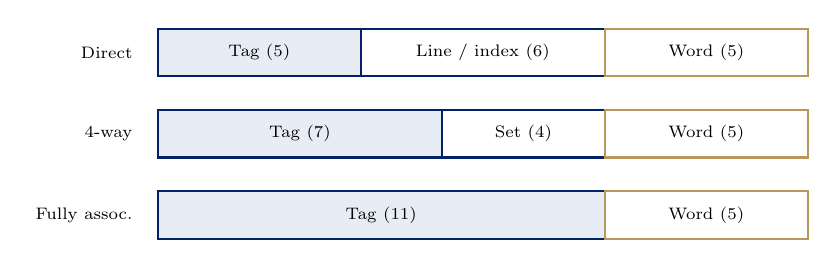
\begin{tikzpicture}[scale=0.86, transform shape,
      every node/.style={font=\scriptsize}]
    % ---- Row 1: direct mapped
    \draw[draw=primary-blue, thick, fill=light-bg] (0,2.05) rectangle (3.0,2.75);
    \draw[draw=primary-blue, thick, fill=white]    (3.0,2.05) rectangle (6.6,2.75);
    \draw[draw=primary-gold, thick, fill=white]    (6.6,2.05) rectangle (9.6,2.75);
    \node at (1.5,2.4) {Tag (5)};
    \node at (4.8,2.4) {Line / index (6)};
    \node at (8.1,2.4) {Word (5)};
    \node[anchor=east] at (-0.25,2.4) {Direct};
    % ---- Row 2: 4-way set associative
    \draw[draw=primary-blue, thick, fill=light-bg] (0,0.85) rectangle (4.2,1.55);
    \draw[draw=primary-blue, thick, fill=white]    (4.2,0.85) rectangle (6.6,1.55);
    \draw[draw=primary-gold, thick, fill=white]    (6.6,0.85) rectangle (9.6,1.55);
    \node at (2.1,1.2) {Tag (7)};
    \node at (5.4,1.2) {Set (4)};
    \node at (8.1,1.2) {Word (5)};
    \node[anchor=east] at (-0.25,1.2) {4-way};
    % ---- Row 3: fully associative
    \draw[draw=primary-blue, thick, fill=light-bg] (0,-0.35) rectangle (6.6,0.35);
    \draw[draw=primary-gold, thick, fill=white]    (6.6,-0.35) rectangle (9.6,0.35);
    \node at (3.3,0.0) {Tag (11)};
    \node at (8.1,0.0) {Word (5)};
    \node[anchor=east] at (-0.25,0.0) {Fully assoc.};
  \end{tikzpicture}
  \caption{One 16-bit address, split three ways (System A: 64~KB memory, 2~KB cache, 32-byte blocks). The word field never moves; the index and tag share a fixed budget of 11 bits.}
  \label{fig:three-splits}
\end{figure}

\textbf{How to present Figure~\ref{fig:three-splits}.} The coordinate map fixes the word-field boundary at $x = 6.6$ across all three rows, and that alignment \emph{is} the teaching point --- so draw it in an order that makes the alignment visible rather than incidental. \emph{Draw the three word fields first}, one under the other, as three identical right-hand boxes, and say: ``block size is 32 bytes in all three schemes, so this field is 5 bits in all three and it is the same 5 bits.'' Only then draw the internal divider in each row --- at the two-thirds point for direct, further right for 4-way, and absent entirely for fully associative. Label the tag widths (5, 7, 11) \emph{last}, all three at once, so students see the tag growing as the divider slides right. If you draw row-by-row instead, the alignment reads as a coincidence and the punchline is lost.

\subsection*{Direct mapping}

Block $B$ may occupy \emph{exactly one} line: $\text{line} = B \bmod L$ and $\text{tag} = \lfloor B/L \rfloor$, where $L$ is the number of lines. The line number is read straight out of the address --- no search, no choice (Stallings 11e, Fig.~5.7, PDF p.~190). Blocks $B$, $B+L$, $B+2L$, \dots\ all land on the same line and are distinguished \emph{only} by the tag.

\begin{figure}[h]
  \centering
  % P7a: block boxes span x -1.0..1.0, line boxes span x 5.0..7.0; both
  % arrows live entirely in the empty corridor x 1.0..5.0, crossing no box.
  % P7b: the horizontal arrow's label sits 0.35 above it; the diagonal's
  % label sits 0.35 below the diagonal's own y at that x (computed in the
  % comment on each \node below).
  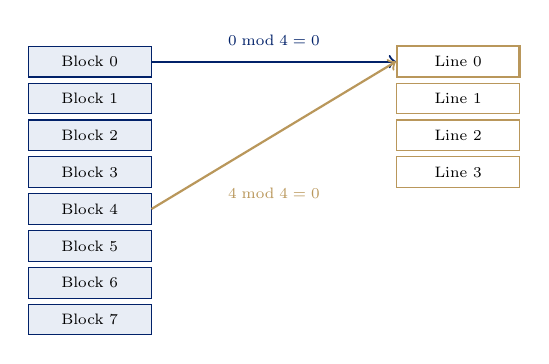
\begin{tikzpicture}[scale=0.78, transform shape,
      every node/.style={font=\scriptsize}]
    \node[draw=primary-blue, fill=light-bg, minimum width=2.0cm,
          minimum height=0.5cm] (B0) at (0,3.5)  {Block 0};
    \node[draw=primary-blue, fill=light-bg, minimum width=2.0cm,
          minimum height=0.5cm]       at (0,2.9)  {Block 1};
    \node[draw=primary-blue, fill=light-bg, minimum width=2.0cm,
          minimum height=0.5cm]       at (0,2.3)  {Block 2};
    \node[draw=primary-blue, fill=light-bg, minimum width=2.0cm,
          minimum height=0.5cm]       at (0,1.7)  {Block 3};
    \node[draw=primary-blue, fill=light-bg, minimum width=2.0cm,
          minimum height=0.5cm] (B4) at (0,1.1)  {Block 4};
    \node[draw=primary-blue, fill=light-bg, minimum width=2.0cm,
          minimum height=0.5cm]       at (0,0.5)  {Block 5};
    \node[draw=primary-blue, fill=light-bg, minimum width=2.0cm,
          minimum height=0.5cm]       at (0,-0.1) {Block 6};
    \node[draw=primary-blue, fill=light-bg, minimum width=2.0cm,
          minimum height=0.5cm]       at (0,-0.7) {Block 7};
    \node[draw=primary-gold, thick, fill=white, minimum width=2.0cm,
          minimum height=0.5cm] (L0) at (6.0,3.5) {Line 0};
    \node[draw=primary-gold, fill=white, minimum width=2.0cm,
          minimum height=0.5cm]       at (6.0,2.9) {Line 1};
    \node[draw=primary-gold, fill=white, minimum width=2.0cm,
          minimum height=0.5cm]       at (6.0,2.3) {Line 2};
    \node[draw=primary-gold, fill=white, minimum width=2.0cm,
          minimum height=0.5cm]       at (6.0,1.7) {Line 3};
    \draw[->, thick, primary-blue] (B0.east) -- (L0.west);
    \draw[->, thick, primary-gold] (B4.east) -- (L0.west);
    % horizontal arrow runs at y=3.5; label 0.35 above it
    \node[primary-blue] at (3.0,3.85) {$0 \bmod 4 = 0$};
    % diagonal descends to y=1.82 at the label's left edge (x=2.2), so the
    % label's top edge must stay below that: top 1.48 => centre 1.35,
    % leaving 0.35 clearance from the line across the whole label width
    \node[primary-gold] at (3.0,1.35) {$4 \bmod 4 = 0$};
  \end{tikzpicture}
  \caption{Many-to-one collision under direct mapping, drawn for a toy cache of $L = 4$ lines. Blocks $0, 4, 8, 12, \dots$ are all forced onto line~0; only one may be resident, and the tag records which.}
  \label{fig:collide}
\end{figure}

\textbf{How to present Figure~\ref{fig:collide}.} Draw the eight block boxes down the left first, numbered, then the \emph{four} line boxes on the right --- and pause on the asymmetry before any arrow exists: eight candidates, four containers. Then draw only \emph{two} arrows, block~0 and block~4, both landing on line~0, and write the modulo arithmetic beside each. Resist drawing all eight arrows; the deck's diagram deliberately omits them because eight crossing arrows teach nothing that two do not. Finish by asking what happens if the program alternates between block~0 and block~4 --- and let the class say ``they keep evicting each other'' rather than saying it yourself. That is the conflict-miss definition, discovered instead of announced.

\begin{teachingaside}
\textbf{The misconception that costs marks:} students conclude from this figure that direct mapping is simply bad. Correct it on the spot --- direct mapping needs \emph{one} comparator of \emph{five} bits, so it is the fastest and cheapest scheme by a wide margin, and its weakness is narrow and specific: two hot blocks that happen to be exactly $L$ apart. On workloads without that pathology it is excellent. Exams reward the trade-off answer, never the ``associativity is better'' answer.
\end{teachingaside}

\textbf{Board:} \textit{(Example 1 of 2 for mapping --- a fresh system, direct mapped.)} Do \emph{not} reuse the deck's System A; students already have that trace. Introduce \key{System B}: main memory $1$~MB, cache $16$~KB, block size $64$~bytes, probe address \texttt{0xA5C7C}. \emph{On the board, in order:} (i) address width, $1\text{ MB} = 2^{20} \Rightarrow N = 20$ bits; (ii) word field, $64 = 2^6 \Rightarrow b = 6$; (iii) lines, $L = 2^{14}/2^{6} = 2^{8} = 256 \Rightarrow$ index $= 8$; (iv) tag $= 20 - 8 - 6 = 6$; (v) the check $6 + 8 + 6 = 20$ \good{\checkmark} --- write the check every single time, and say that a student who writes it will catch most of their own errors. Only then slice the address. Write \texttt{0xA5C7C} in binary as $1010\,0101\,1100\,0111\,1100$ and cut it $6\mid 8\mid 6$:
\begin{itemize}
  \item Tag $= 101001_2 = 41$, \quad Index $= 01110001_2 = 113$, \quad Word $= 111100_2 = 60$.
\end{itemize}
Then verify by the \emph{other} route, arithmetic rather than bit-slicing, exactly as the deck insists: $\texttt{0xA5C7C} = 679036$; block $B = \lfloor 679036/64 \rfloor = 10609$; offset $= 679036 - 10609\times 64 = 60$ \good{\checkmark}; line $= 10609 \bmod 256 = 113$ \good{\checkmark}; tag $= \lfloor 10609/256 \rfloor = 41$ \good{\checkmark}. Two independent routes, same answer --- that is the exam technique you are actually teaching.

\subsection*{Fully associative and $k$-way set associative}

Fully associative mapping removes the index entirely: a block may occupy \emph{any} line, so the tag must be the whole block number ($N - b$ bits) and every line's tag must be compared in parallel. Maximum placement freedom, maximum identification cost. $k$-way set associative is the compromise: group the $L$ lines into $S = L/k$ \key{sets}; the index selects one set, and the block may occupy any of the $k$ ways within it, so $k$ comparators suffice.

\begin{figure}[h]
  \centering
  %   (11.5,1.9)->(13.2,1.9) horizontal in the empty corridor x 11.5..13.2.
  % P7b: each edge label sits >= 0.3 units (0.186 cm at scale 0.62) off its
  %      own line, never on it.
  % P7c: every unboxed label clears the nearest box edge by >= 0.25 units
  %      (0.155 cm at scale 0.62).
  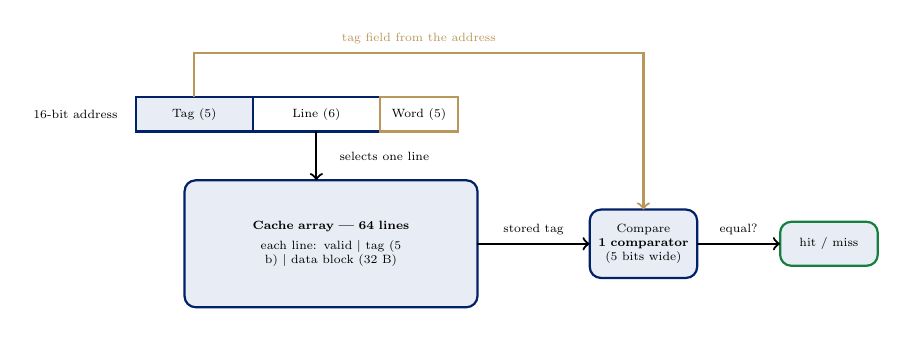
\begin{tikzpicture}[scale=0.62, transform shape,
      every node/.style={font=\scriptsize}]
    \draw[draw=primary-blue, thick, fill=light-bg] (0,4.2) rectangle (2.4,4.9);
    \draw[draw=primary-blue, thick, fill=white]    (2.4,4.2) rectangle (5.0,4.9);
    \draw[draw=primary-gold, thick, fill=white]    (5.0,4.2) rectangle (6.6,4.9);
    \node at (1.2,4.55) {Tag (5)};
    \node at (3.7,4.55) {Line (6)};
    \node at (5.8,4.55) {Word (5)};
    \node[anchor=east] at (-0.25,4.55) {16-bit address};
    \node[draw=primary-blue, thick, fill=light-bg, rounded corners,
          minimum width=6.0cm, minimum height=2.6cm, text width=5.5cm,
          align=center]
          (ARR) at (4.0,1.9)
          {\textbf{Cache array --- 64 lines}\\[0.12cm]
           each line: valid $\mid$ tag (5 b) $\mid$ data block (32 B)};
    \node[draw=primary-blue, thick, fill=light-bg, rounded corners,
          minimum width=2.2cm, minimum height=1.4cm, text width=1.9cm,
          align=center]
          (CMP) at (10.4,1.9) {Compare\\\textbf{1 comparator}\\(5 bits wide)};
    \node[draw=positive, thick, fill=light-bg, rounded corners,
          minimum width=2.0cm, minimum height=0.9cm, align=center]
          (HIT) at (14.2,1.9) {hit / miss};
    \draw[->, thick] (3.7,4.2) -- (3.7,3.2);
    \node[anchor=west] at (4.05,3.7) {selects one line};
    \draw[->, thick] (7.0,1.9) -- (9.3,1.9);
    \node at (8.15,2.20) {stored tag};
    \draw[->, thick, primary-gold] (1.2,4.9) -- (1.2,5.8) -- (10.4,5.8) -- (10.4,2.6);
    \node[primary-gold] at (5.80,6.10) {tag field from the address};
    \draw[->, thick] (11.5,1.9) -- (13.2,1.9);
    \node at (12.35,2.20) {equal?};
  \end{tikzpicture}
  \caption{Direct-mapped hardware. The line field is a \emph{decoder input}, not something searched for; only after a line is selected does a single comparison decide hit or miss.}
  \label{fig:direct-hw}
\end{figure}

\begin{figure}[h]
  \centering
  %   (1.5,4.9)->(1.5,5.8)->(10.0,5.8)->(10.0,3.2) : the y=5.8 leg is above
  %       every box; the x=10.0 drop is right of the array (east edge 7.0)
  %       and lands on the comparator block's top edge.
  %   (11.1,1.9)->(12.4,1.9) : empty corridor.
  % P7b: "4 stored tags" sits at (7.95,3.15), 0.35 above the topmost of the
  %       four horizontals (y=2.8) and outside both boxes in x.
  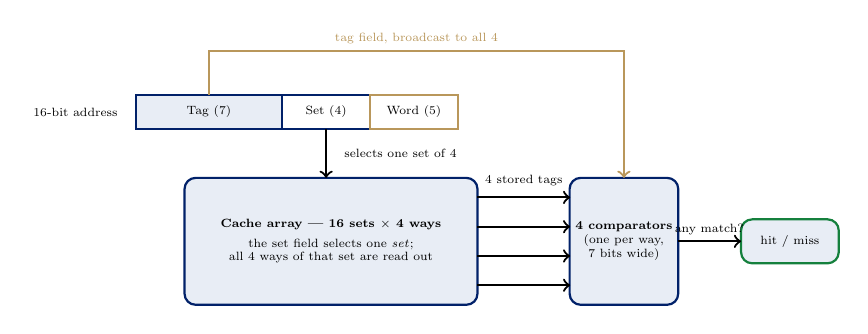
\begin{tikzpicture}[scale=0.62, transform shape,
      every node/.style={font=\scriptsize}]
    \draw[draw=primary-blue, thick, fill=light-bg] (0,4.2) rectangle (3.0,4.9);
    \draw[draw=primary-blue, thick, fill=white]    (3.0,4.2) rectangle (4.8,4.9);
    \draw[draw=primary-gold, thick, fill=white]    (4.8,4.2) rectangle (6.6,4.9);
    \node at (1.5,4.55) {Tag (7)};
    \node at (3.9,4.55) {Set (4)};
    \node at (5.7,4.55) {Word (5)};
    \node[anchor=east] at (-0.25,4.55) {16-bit address};
    \node[draw=primary-blue, thick, fill=light-bg, rounded corners,
          minimum width=6.0cm, minimum height=2.6cm, align=center]
          (ARR) at (4.0,1.9)
          {\textbf{Cache array --- 16 sets $\times$ 4 ways}\\[0.12cm]
           the set field selects one \emph{set};\\
           all 4 ways of that set are read out};
    \node[draw=primary-blue, thick, fill=light-bg, rounded corners,
          minimum width=2.2cm, minimum height=2.6cm, align=center]
          (CMP) at (10.0,1.9) {\textbf{4 comparators}\\(one per way,\\7 bits wide)};
    \node[draw=positive, thick, fill=light-bg, rounded corners,
          minimum width=2.0cm, minimum height=0.9cm, align=center]
          (HIT) at (13.4,1.9) {hit / miss};
    \draw[->, thick] (3.9,4.2) -- (3.9,3.2);
    \node[anchor=west] at (4.15,3.7) {selects one set of 4};
    \draw[->, thick] (7.0,2.8) -- (8.9,2.8);
    \draw[->, thick] (7.0,2.2) -- (8.9,2.2);
    \draw[->, thick] (7.0,1.6) -- (8.9,1.6);
    \draw[->, thick] (7.0,1.0) -- (8.9,1.0);
    \node at (7.95,3.15) {4 stored tags};
    \draw[->, thick, primary-gold] (1.5,4.9) -- (1.5,5.8) -- (10.0,5.8) -- (10.0,3.2);
    \node[primary-gold] at (5.75,6.05) {tag field, broadcast to all 4};
    \draw[->, thick] (11.1,1.9) -- (12.4,1.9);
    \node at (11.75,2.15) {any match?};
  \end{tikzpicture}
  \caption{4-way set-associative hardware. Identical skeleton to Figure~\ref{fig:direct-hw}: one comparator becomes $k$, and two bits move from the index field into the tag.}
  \label{fig:setassoc-hw}
\end{figure}

\textbf{How to present Figures~\ref{fig:direct-hw} and~\ref{fig:setassoc-hw} --- as one drawing, twice.} These two figures share a skeleton deliberately, and the pedagogy only works if you exploit that. \emph{Draw Figure~\ref{fig:direct-hw} once and do not erase it.} Its build order, from the coordinate map: the address strip along the top first; then the big cache-array box below it; then the vertical arrow down from the \emph{index} field into the array, narrating ``the index is a decoder input --- it \emph{selects}, it does not search''; then the comparator box to the right; then the long gold path carrying the \emph{tag} field over the top of the array and down into the comparator --- draw that one last and slowly, because the whole architecture is in it: index goes down into the array, tag goes across into the comparator. Finish with the hit/miss box.

Then, for Figure~\ref{fig:setassoc-hw}, \emph{modify rather than redraw}. Change three things in front of the class: slide the tag/index divider two bits to the right ($5\mid 6$ becomes $7\mid 4$); relabel the array ``16 sets $\times$ 4 ways''; and replace the single comparator with a stack of four, adding the four horizontal tag lines. Everything else stays. Say explicitly: ``associativity did not change the architecture, only the width of two fields and the number of comparators.'' Students who see the two diagrams drawn independently memorise two pictures; students who watch one morph into the other understand one dial.

\begin{teachingaside}
\textbf{Live-interaction hook, placed here.} Before you add the fourth comparator, ask: ``comparators cost area and sit on the critical path. If 4-way needs 4, and fully associative on this 64-line cache needs 64 --- what does the tag storage do over the same range?'' Take guesses. Most students expect tag storage to blow up proportionally too. The answer is that it grows by only \emph{one bit per line} per doubling of $k$: $320$ bits at direct, $448$ at 4-way, $704$ fully associative --- a mere $2.2\times$, against a $64\times$ explosion in comparators. \key{It is the comparators, not the tag bits, that make full associativity unaffordable.} That inversion of expectation is the single most memorable thing in Act~4.
\end{teachingaside}

\textbf{Board:} \textit{(Example 2 of 2 for mapping --- System B again, now 8-way.)} Keep System B on the board and change only the associativity: $1$~MB memory, $16$~KB cache, $64$-byte blocks, now \key{8-way set associative}, same probe address \texttt{0xA5C7C}. \emph{On the board, in order:} (i) note what is \emph{unchanged} --- $N = 20$, $b = 6$, $L = 256$ --- and say aloud that neither address width nor block size nor line count depends on associativity; (ii) sets, $S = L/k = 256/8 = 32 \Rightarrow$ index $= 5$ bits; (iii) tag $= 20 - 5 - 6 = 9$ bits; (iv) the check, $9 + 5 + 6 = 20$ \good{\checkmark}. Then slice the same binary string $1010\,0101\,1100\,0111\,1100$ as $9\mid 5\mid 6$: tag $= 101001011_2 = 331$, set $= 10001_2 = 17$, word $= 111100_2 = 60$. Cross-check arithmetically from $B = 10609$: set $= 10609 \bmod 32 = 17$ \good{\checkmark}, tag $= \lfloor 10609/32 \rfloor = 331$ \good{\checkmark}. Finally point at the two results side by side: going from direct ($k=1$) to 8-way, the index lost exactly $3$ bits and the tag gained exactly $3$ --- and the word field never moved. \key{Doubling $k$ always trades one index bit for one tag bit.} If students take one transferable rule from Act~4, make it that one.

\section{Topic 5: Replacement Algorithms}

The second GATE-load-bearing act. Open by narrowing the question sharply, because students over-apply replacement: \emph{under direct mapping there is no decision to make at all} --- the incoming block has exactly one legal line, and whatever is there is evicted. A replacement policy is needed only when the block has a \emph{choice} of homes: fully associative (choose among all $L$ lines) or $k$-way set associative (choose among the $k$ ways of one set). Getting students to say that back to you is worth the thirty seconds.

The five policies, in the order the deck presents them:

\begin{itemize}
  \item \key{FIFO} --- evict the block that has been resident longest, regardless of use. Tracks load order only.
  \item \key{LRU} --- evict the block unused for the longest time. Tracks recency.
  \item \key{LFU} --- evict the block with the smallest reference count. Tracks frequency.
  \item \key{Random} --- evict an arbitrary block. Tracks nothing.
  \item \key{OPT} (Belady's MIN) --- evict the block whose \emph{next} use is furthest in the future. Requires the future; unimplementable, and used only as a benchmark.
\end{itemize}

\begin{teachingaside}
\textbf{Sourcing, stated out loud.} Stallings 11e covers LRU, FIFO, LFU, and Random only. OPT and Belady's anomaly are standard general treatment carried in no page of our anchor text --- present them as such, and if pressed, point students to an operating-systems text's page-replacement chapter. Modelling this honesty is part of the lecture, not an interruption to it.
\end{teachingaside}

The deck runs all five against one common reference string ($7, 0, 1, 2, 0, 3, 0, 4, 2, 3, 0, 3, 2$ on a 3-line fully associative cache) and gets $3$, $4$, $5$, $3$, and $6$ hits respectively --- FIFO, LRU, LFU, Random, OPT. Walk at least FIFO and LRU live; the others can be shown as completed tables. The headline is the spread: identical input, identical cache, and a \key{$2\times$ range in hit ratio} from $23.1\%$ to $46.2\%$. The policy is not a detail.

\begin{teachingaside}
\textbf{The misconception that matters most in this act:} that LRU is simply the best implementable policy. On the deck's string LFU beats it ($5$ hits versus $4$), and the board example below shows a string where even \emph{FIFO} beats LRU outright. Say the honest version: no implementable policy dominates on all strings; LRU is preferred in practice because it is robust across \emph{typical} workloads and cheap at low associativity, not because it wins every trace. Students who learn ``LRU is best'' will confidently mis-answer any exam question engineered around a counterexample --- and examiners engineer them precisely because the misconception is so common.
\end{teachingaside}

\textbf{Board:} \textit{(Example 1 of 2 for replacement --- a fresh string where FIFO beats LRU.)} Use a $3$-line fully associative cache, initially empty, and the string
\[ 2,\;3,\;4,\;2,\;5,\;3,\;4,\;5,\;2,\;3 \qquad (10\text{ references}). \]
\emph{On the board, in order:} draw the reference row across the top first; then three empty slot rows beneath it; then a hit/miss row at the bottom --- the empty grid before any content, so students can copy the frame while you fill it. Fill \emph{column by column}, never row by row, narrating the eviction decision at each miss. Run FIFO first:
\begin{itemize}
  \item References $2, 3, 4$: three compulsory misses; queue order is $[2,3,4]$.
  \item Reference $2$: \good{hit} (FIFO does \emph{not} reorder on a hit --- say this aloud, it is the whole difference from LRU).
  \item Reference $5$: miss; evict the queue head $2$; residents $\{3,4,5\}$, queue $[3,4,5]$.
  \item References $3, 4, 5$: three consecutive \good{hits}.
  \item Reference $2$: miss; evict head $3$; residents $\{4,5,2\}$.
  \item Reference $3$: miss; evict head $4$.
  \item \key{FIFO result: 4 hits, 6 misses.}
\end{itemize}
Now re-run the identical string under LRU on a fresh grid: references $2,3,4$ miss; reference $2$ \good{hits} \emph{and promotes $2$ to most-recent}; reference $5$ misses and evicts $3$ (least recently used); reference $3$ misses and evicts $4$; reference $4$ misses and evicts $2$; reference $5$ \good{hits}; reference $2$ misses and evicts $3$; reference $3$ misses and evicts $4$. \key{LRU result: 2 hits, 8 misses} --- half of FIFO's.

\begin{teachingaside}
\textbf{Live-interaction hook --- a prediction trap, and the best one in the lecture.} Before running the LRU pass, tell the class you are about to run the same string under LRU and ask them to commit, by show of hands, to whether LRU will do better, worse, or the same as FIFO's 4 hits. Nearly everyone votes ``better'', because the deck's own common string had LRU beating FIFO. The answer is \emph{worse} --- LRU manages only 2. Let the surprise sit before explaining: reference $2$ at step~4 promotes block $2$ to most-recent under LRU, which pushes block $3$ to the bottom and gets it evicted at step~5 --- just before $3$ is needed at step~6. FIFO, by ignoring the hit entirely, happens to keep the block LRU throws away. \key{Recency is a heuristic about the future, and heuristics can be wrong.}
\end{teachingaside}

\textbf{Board:} \textit{(Example 2 of 2 --- OPT on the same string, to price the heuristics.)} Keep the same $3$-line cache and the same string $2,3,4,2,5,3,4,5,2,3$, and run OPT. \emph{On the board, in order:} at each miss, write the residents' \emph{next-use positions} in a small side column \emph{before} naming the victim --- that side column is the entire method, and students who skip it guess. References $2,3,4$ miss; reference $2$ \good{hits}; at reference $5$ the residents are $\{2,3,4\}$ with next uses at steps $9$, $6$, and $7$ respectively, so block~$2$ (furthest, step~9) is evicted; references $3, 4, 5$ then all \good{hit}; at reference $2$ the residents are $\{5,3,4\}$ and both $5$ and $4$ are never used again, so either may go; reference $3$ \good{hits}. \key{OPT result: 5 hits, 5 misses.} Line the three up on the board --- OPT $5$, FIFO $4$, LRU $2$ --- and close the act: OPT is the ceiling no implementable policy can beat, FIFO got unusually lucky here, LRU got unlucky, and \emph{one string proves nothing about policies in general --- it proves only that policies diverge}, which is why real designs are chosen by simulation over real traces rather than by argument.

\subsection*{Belady's anomaly}

The claim that ought to be impossible: under \key{FIFO}, \emph{increasing} the number of cache lines can \emph{increase} the number of misses on the same string. The deck demonstrates it on the string
\[ 1,\;2,\;3,\;4,\;1,\;2,\;5,\;1,\;2,\;3,\;4,\;5 : \]
with $3$ lines, $9$ misses; with $4$ lines, $10$ misses.

\textbf{How to present it.} Draw both grids \emph{side by side on the same board}, three slots on the left and four on the right, and fill them in lockstep column by column --- reference~1 on both, then reference~2 on both, and so on. The anomaly is invisible if you complete one table and then the other, because by then students have lost the first. Filled in parallel, the divergence is watchable: the 4-line cache is comfortably ahead early (it \good{hits} at references $5$ and $6$ where the 3-line cache misses) and then loses that lead and more over the tail. Write the two totals at the bottom simultaneously and let the class read them off.

Then give the explanation, which is the part exams reward: \key{LRU and OPT are immune} because they are \emph{stack algorithms} --- the set of blocks held with $n$ lines is always a subset of the set held with $n+1$ lines, so extra capacity can never remove a block that would otherwise have hit. FIFO has no such property: adding a line changes the eviction \emph{order} itself, not merely its depth.

Close the act with the hardware cost of each policy, since it explains why the theoretically-best policy is rarely built: LRU on a \emph{two-way} set needs a single USE bit per set; LRU on a fully associative cache needs an $L$-entry recency list reordered on every access --- which is why exact LRU is rare beyond small associativities. FIFO needs a $\lceil \log_2 k \rceil$-bit round-robin pointer per set with no update at all on a hit; LFU needs a counter per line plus a comparison tree, and periodic ageing to stop stale counts dominating; Random needs no per-line state whatsoever. \key{Cost rises with how much history the policy remembers} --- Random remembers nothing, exact LRU remembers everything.

\section{Topic 6: Cache Performance}

The final act puts numbers on everything. Define the terms once, precisely: for $n$ references of which $n_h$ hit, $H = n_h/n$ and the miss ratio is $1 - H$, and
\[
  \text{AMAT} \;=\; T_{\text{hit}} + (1-H)\times T_{\text{miss penalty}} .
\]
Reconcile this with Topic~1's two-level form explicitly, because students think they are different formulas: $T_{\text{avg}} = HT_1 + (1-H)(T_1+T_2)$ expands to $T_1 + (1-H)T_2$, which \emph{is} AMAT with $T_{\text{hit}} = T_1$ and miss penalty $= T_2$. One formula, two spellings.

\begin{teachingaside}
\textbf{The single most common arithmetic error in this act:} treating the miss penalty as the total miss time and adding the hit time twice. A miss penalty is the \emph{extra} time \emph{beyond} the hit time, because the hit time is paid on every access, hit or miss. Give students the sanity test and insist on it: \key{any AMAT answer must lie strictly between the hit time and the full miss time.} An answer outside that interval is wrong without further checking --- and it costs nothing to verify.
\end{teachingaside}

\textbf{Board:} \textit{(Example 1 of 2 --- AMAT from a raw reference count.)} A program makes $5000$ memory references, of which $4600$ hit. Cache access time is $3$~ns; a miss costs a further $120$~ns to fetch the block. \emph{On the board, in order:} hit ratio first, $H = 4600/5000 = 0.92$, and miss ratio $0.08$ beside it; then AMAT $= 3 + 0.08\times 120 = 3 + 9.6 = 12.6$~ns; then the cross-check in the other form, $0.92\times 3 + 0.08\times 123 = 2.76 + 9.84 = 12.6$~ns \good{\checkmark}; then the sanity test last, $3 < 12.6 < 123$ \good{\checkmark}. Doing the cross-check every time is what stops the double-counting error from ever appearing in a script.

Then the two-level case, where a second trap lives. With an L1 (time $t_1$, hit ratio $h_1$), an L2 (time $t_2$, \emph{local} hit ratio $h_2$ measured over L1 misses only), and main memory (time $t_m$), two access models decide the arithmetic:
\[
  \textbf{Hierarchical: } T = h_1t_1 + (1-h_1)h_2(t_1+t_2) + (1-h_1)(1-h_2)(t_1+t_2+t_m),
\]
\[
  \textbf{Simultaneous: } T = h_1t_1 + (1-h_1)h_2\,t_2 + (1-h_1)(1-h_2)\,t_m.
\]
Tell students to read every question for which model is intended, and that absent any statement they should assume hierarchical --- it is what real multi-level caches do.

\textbf{Board:} \textit{(Example 2 of 2 --- both models, and the local/global trap.)} Take $t_1 = 2$~ns with $h_1 = 0.90$; $t_2 = 15$~ns with \emph{local} $h_2 = 0.80$; $t_m = 150$~ns. \emph{On the board, in order:} draw the three-case probability tree first --- L1 hit / L1 miss \& L2 hit / both miss --- and write the three probabilities $0.90$, $0.08$, $0.02$ on its branches \emph{before} any time appears; then attach the hierarchical times to each branch; then sum; and write the weight check last.
\begin{itemize}
  \item L1 hit: $0.90 \times 2 = 1.8$~ns.
  \item L1 miss, L2 hit: $0.10\times 0.80\times(2+15) = 0.08\times 17 = 1.36$~ns.
  \item Both miss: $0.10\times 0.20\times(2+15+150) = 0.02\times 167 = 3.34$~ns.
  \item \key{Hierarchical total: $T = 1.8 + 1.36 + 3.34 = 6.5$~ns.} Weight check: $0.90+0.08+0.02 = 1.000$ \good{\checkmark}.
  \item Simultaneous, same numbers: $0.90(2) + 0.08(15) + 0.02(150) = 1.8+1.2+3.0 = \key{6.0}$~ns.
\end{itemize}
Then spring the trap explicitly, because it is a full-marks error rather than a rounding one: here $h_2 = 0.80$ is \emph{local} --- $80\%$ of the references that \emph{reach} L2. The \key{global} L2 hit ratio is $(1-h_1)h_2 = 0.10\times 0.80 = 0.08$, i.e.\ only $8\%$ of all references. Teach students the linguistic tell: the phrase ``of the accesses that miss in L1'' marks a \emph{local} ratio; ``of all memory references'' marks a \emph{global} one. If a problem states neither, say which you assumed.

\begin{teachingaside}
\textbf{Live-interaction hook to close the lecture.} Pose the budget question and take a vote before revealing anything. Starting from $t_1 = 1$~ns, $h_1 = 0.95$, $t_m = 100$~ns and no L2 --- so $\text{AMAT} = 1 + 0.05\times100 = 6$~ns --- you may spend your entire budget on exactly one of: (a) halving the hit time to $0.5$~ns, or (b) raising the hit ratio to $0.975$. Most classes vote (a), because halving \emph{feels} like the bigger intervention. The arithmetic: (a) gives $0.5 + 0.05\times100 = 5.5$~ns, a $0.5$~ns saving; (b) gives $1 + 0.025\times100 = 3.5$~ns, a $2.5$~ns saving --- \key{five times better}. The lesson, and the last thing to leave on the board: when the miss penalty is large, the miss \emph{rate} dominates AMAT and the hit time is a second-order term. That is precisely why the lecture spent its two longest acts on mapping and replacement --- both are miss-rate levers.
\end{teachingaside}

\section{Summary --- One-Page Pre-Class Refresh}

\begin{itemize}
  \item \textbf{Why a hierarchy:} fast / large / cheap cannot be had together; locality (temporal $\to$ keep a block, spatial $\to$ fetch a whole block) makes a layered organisation work. Two-level model: $T_{\text{avg}} = T_1 + (1-H)T_2$. $H$ is an outcome, not a knob.
  \item \textbf{Main memory:} SRAM (flip-flop, no refresh, fast, dear $\to$ cache) versus DRAM (capacitor, refresh needed, dense, cheap $\to$ main memory); both volatile. ROM family in order of flexibility: mask ROM, PROM, EPROM, EEPROM, flash (block erase --- hence SSDs).
  \item \textbf{Cache vocabulary:} block (unit in memory) $=$ line (container in cache) in size; tag identifies which block a line holds; valid bit says whether it holds anything. A miss fetches the \emph{whole block}.
  \item \textbf{Master framework:} $\text{tag} = N - \text{index} - b$, and the three fields always re-sum to $N$. Word field is fixed by block size and never moves. Doubling $k$ trades one index bit for one tag bit.
  \item \textbf{Mapping:} direct ($\text{line} = B \bmod L$, $\text{tag} = \lfloor B/L \rfloor$, 1 comparator, conflict misses); fully associative (no index, tag $=$ block number, $L$ comparators, needs replacement); $k$-way (index selects one of $S = L/k$ sets, $k$ comparators). System A ($64$~KB / $2$~KB / $32$~B, address \texttt{0x3F8C}): direct $\to$ tag $7$, line $60$, word $12$; 4-way $\to$ tag $31$, set $12$; fully $\to$ tag $508$. Cost: comparators double with $k$, tag storage grows only one bit per line --- comparators are the binding constraint.
  \item \textbf{Replacement} (needed only where a block has a choice of homes): FIFO, LRU, LFU, Random, OPT. On the deck's string: $3/4/5/3/6$ hits respectively. No implementable policy dominates on all strings. Belady's anomaly --- more FIFO lines can mean more misses ($9$ at 3 lines, $10$ at 4); LRU and OPT are immune because they are stack algorithms. Hardware cost rises with remembered history: Random (nothing) $\to$ FIFO (pointer) $\to$ LRU (USE bit at 2-way; full list otherwise) $\to$ LFU (counters $+$ ageing).
  \item \textbf{Performance:} $\text{AMAT} = T_{\text{hit}} + (1-H)T_{\text{miss penalty}}$; miss penalty is the \emph{extra} time; answer must lie between hit time and full miss time. Two-level: hierarchical (times add) versus simultaneous (only the answering level counts); assume hierarchical unless told otherwise. Local versus global L2 hit ratio is a full-marks distinction. Miss rate beats hit time when the penalty is large.
  \item \textbf{Citation discipline to hold at the board:} Stallings 11e Ch.~4 / Ch.~5 \S\S5.1--5.2 / Ch.~6 \S6.1 are page-citable; P\&H \S5.3 (p.~397) for AMAT; Hamacher Ch.~8 chapter-level only; \key{OPT and Belady's anomaly get no page citation at all} --- they are not in our anchor text.
  \item \textbf{Bridge to Week 10:} the same block-placement question, asked one level down --- pages instead of blocks, main memory instead of cache, plus associative memory, segmentation, and secondary storage.
\end{itemize}

\end{document}
